\documentclass[12pt]{article}

\usepackage{graphicx,url}

\usepackage[brazilian]{babel}
\usepackage[utf8x]{inputenc}
\usepackage{amssymb,amsmath}
\usepackage[T1]{fontenc}
\usepackage{verbatim}
\usepackage{hyperref}
\usepackage{fullpage}
\usepackage{multicol}
\usepackage{lmodern}
\usepackage{xcolor}
\usepackage{listings}
\usepackage[colorinlistoftodos]{todonotes}
\usepackage{fixltx2e}
\usepackage{longtable}
\usepackage{float}
\usepackage{wrapfig}
\usepackage{soul}
\usepackage{textcomp}
\usepackage{marvosym}
\usepackage{wasysym}
\usepackage{latexsym}
\usepackage{amssymb}
\usepackage{hyperref}
\tolerance=1000
\usepackage{geometry}
\geometry{left=0.7in,right=0.7in,top=1in,bottom=1in}
\providecommand{\alert}[1]{\textbf{#1}}


\graphicspath { {figures/} }
\setlength{\parindent}{0cm}
% Algum problema em manter o \parindent em zero? Eu particularmente não gosto da indentação e normalmente pulo uma
% linha extra entre os paragrafos. --GraphGenerator


\title{Grande Organizador de Dados (GOD) \\Great Data Organizer}
\author{
Programação Orientada a Objetos (MAC0441/5714)\\
Departamento Ciência da Computação -- DCC\\
Instituto de Matemática e Estatística -- IME\\
Universidade de Sao Paulo -- USP
}
\date{Dezembro, 2014}

\begin{document}
\maketitle
\newpage
\tableofcontents
\newpage

\section{Introdução}
Grande Organizador de Dados (GOD) é um sistema composto por módulos que realizam a entrada e saída de diversas fontes de informação, como arquivos texto, planilhas, html, emails e redes sociais, entre outros. 
Essas informações podem ser utilizadas para a criação de aplicações que fazem a análise de dados de diferentes formas, como análise de sentimentos e agregadores de informações.
O GOD foi desenvolvido em Smalltalk pelos alunos da disciplina de Programação Orientada a Objetos. A seguir são descritas as principais funcionalidades dos módulos e das aplicações do GOD.


\section{Funcionalidades principais}

\subsection{Módulos}

\subsubsection{Kernel}
\begin{enumerate}
\item Fornecer uma estrutura de dados básica para a manipulação das diferentes fontes de informação. A classe GODData representa essa estrutura, que é estendida pelos demais módulos para atender suas especificidades.
\item Gerenciar o versionamento do projeto.
\end{enumerate}

\subsubsection{Banco de dados}
\begin{enumerate}
\item Armazenamento de objetos
\item Realização de consultas sobre objetos armazenados
\item Gerenciamento do servidor
\item Gerenciamento de conexões de clientes
\end{enumerate}

\subsubsection{E-mails}
\begin{enumerate}
\item Recebimento de e-mails utilizando uma conexão segura
\item Envio de e-mails utilizando uma conexão segura
\end{enumerate}

\subsubsection{Filtros}
\begin{enumerate}
\item Filtragem de dados por título
\item Filtragem de dados por conteúdo
\item Filtragem de dados por origem
\item Filtragem de dados por tags
\item Filtragem de string por marcadores de texto (por exemplo tags html)
\end{enumerate}

\subsubsection{Gráficos}
\begin{enumerate}
\item Geração de gráfico de barras no formato PNG
\item Geração de gráfico de barras no Squeak (Morph)
\item Geração de gráfico de linhas no formato PNG
\item Geração de gráfico de linhas no Squeak (Morph)
\end{enumerate}

\subsubsection{Páginas web}
\begin{enumerate}
\item Criação de aplicações web
\item Leitura de páginas HTML
\end{enumerate}

\subsubsection{Planilhas}
\begin{enumerate}
\item Leitura e escrita em CSV
\item Leitura e escrita em ODS
\item Leitura em XLSX
\item Junção de duas planilhas
\item Geração de planilhas a partir de dicionários e listas
\end{enumerate}

\subsubsection{Processadores}
\begin{enumerate}
\item Geração de tags relevantes. As tags são obtidas a partir de conteúdo de texto de entrada de acordo com a sua relevância usando o algoritmo de recuperação de informação tf-idf.
\item Cálculo de média, mediana, variância e desvio padrão para dados numéricos
\end{enumerate}

\subsubsection{Redes sociais}
Facebook
\begin{enumerate}
\item Busca de usuários
\item Busca por posts de usuário
\item Filtragem dos posts
\item Busca de páginas
\item Busca por grupos
\end{enumerate}

Twitter
\begin{enumerate}
\item Busca na timeline
\item Busca por hashtags
\item Busca de tweets
\item Filtragem por data e por língua
\item Realizar buscas avançadas:
\begin{enumerate}
\item Busca contendo todas as palavras
\item Busca por qualquer uma das palavras
\item Busca pela frase exata
\item Busca por qualquer hashtag
\item Busca por todas as hashtags
\item Busca contendo nenhuma das palavras
\end{enumerate}
\end{enumerate}

\subsubsection{Textos}
\begin{enumerate}
\item Leitura e escrita em ODT
\item Leitura e escrita em TXT
\item Leitura e escrita em RTF
\item Leitura e escrita em PDF
\end{enumerate}

\subsection{Aplicações}

\subsubsection{Agregação de conferências}
\begin{enumerate}
\item Busca por conferências
\item Agregação de informações sobre conferências
\item Leitura de dados do ConfSearch
\item Leitura de dados do WIKICFP
\item Leitura de dados do Qualis
\item Geração de planilha com as conferências resultantes da busca
\item Geração de palavras-chave para conferências
\end{enumerate}

\subsubsection{Agregação de informações acadêmicas}
\begin{enumerate}
\item Busca por pesquisadores a partir de perfis do Google Scholar
\item Cálculo de estatísticas sobre um pesquisador
\item Geração de gráfico de fator de impacto e quantidade de artigos publicados
\end{enumerate}

\subsubsection{Análise de sentimento de consumo}
\begin{enumerate}
\item Contagem de palavras positivas, neutras ou negativas em textos
\item Saída da análise em gráfico
\item Saída da análise em planilha
\end{enumerate}

\subsubsection{Análise de sentimento político}
\begin{enumerate}
\item Contagem de palavras positivas, neutras ou negativas sobre candidatos ou partidos
\item Validação de dados do TSE sobre candidatos e partidos
\item Saída da análise em gráfico
\item Saída da análise em planilha
\end{enumerate}

\newpage
% \def\godkernel{\textbf{GODKernel}}
\def\goddata{\textbf{GODData}}
\def\configGod{\textbf{ConfigurationOfGOD}}

\section{Núcleo (\godkernel)}

\godkernel~ é o módulo que contém a classe que representa a estrutura básica para manipulação de dados do projeto.
Essa classe é chamada \goddata~ contém os atributos para armazenamento comuns aos diferentes tipos de fontes de dados usados no projeto. 
\goddata~ pode ser estendido para atender às especificidades dessas diferentes fontes de informações.\\
Esse módulo também é responsável por gerenciar o repositório do projeto, realizando o controle de versões e suas dependências.\\
Em caso de dúvidas, entre em contato com \emph{Higor: hamario [at] ime.usp.br}.


\subsection{\goddata} 

Classe que representa a estrutura básica a serem armazenadas das diferentes fontes de informação, comoarquivos texto, planilhas, páginas html, redes sociais,e-mails, entre outras.

\subsubsection{Atributos}

\begin{itemize}
 \item \textbf{author} - autor de um conteúdo.
 \item \textbf{content} - armazena o conteúdo principal de uma fonte de informação.
 \item \textbf{height} - altura do objeto a ser renderizado.
 \item \textbf{id} - valor exclusivo do objeto.
 \item \textbf{layoutGrid} - matriz que contém objetos \goddata~ internos. Atributo que representa a posição na qual os objetos internos devem ser renderizados em uma página web.
 \item \textbf{origin} - origem da informação.
 \item \textbf{tags} - termos principais associados ao objeto \goddata.
 \item \textbf{timestamp} - data do \goddata.
 \item \textbf{title} - Titulo da informação.
 \item \textbf{width} - largura do objeto a ser renderizado.
\end{itemize}


\subsubsection{Métodos}

\begin{itemize}
 \item \textbf{addOnLayoutGrid:a\goddata~ at: aRow at: aColumn} - adiciona um \goddata~ ao layoutGrid.
 \item \textbf{addTag:} - adiciona uma nova tag à coleção de tags.
 \item \textbf{is\goddata} - verifica se um objeto é do tipo \goddata.
 \item \textbf{isWho} - informa o tipo de subclasse de \goddata.
 \item \textbf{layoutGridRowSize: rowNumber columnSize: columnNumber} - define as dimensões do layoutGrid.
 \item \textbf{tagExists:} - verifica se uma determinada tag existe.
\end{itemize}


\subsubsection{Exemplos}

\begin{godCode}
'Preenchendo um \goddata'
goddata := \godData~ new.
goddata title:'titulo do objeto'.
goddata author:'proprietario da informacao'
goddata content: 'Conteudo que faz parte da informacao'
goddata addTag: 'termo'.

'Definindo o tamanho do layoutGrid e atribuindo objetos \goddata~ a este grid'
goddata {layoutGridRowSize: 5 columnSize: 3.
goddata addOnLayoutGrid: godddata1 at: 1 at: 1.
goddata addOnLayoutGrid: godddata1 at: 3 at: 3.

'Adicionando uma tag a colecao'
goddata addTag: 'termo'.

\end{godCode}


\subsection{\configGod} 

Classe responsável pelo gerenciamento dos módulos do projeto. Possui módulos para fazer o download de versões dos módulos e dependências do projeto, assim como a realização de backup do repositório.

\subsubsection{Métodos}

\begin{itemize}
 \item \textbf{backupPackages:} - realiza o backup dos módulos do projeto.
 \item \textbf{baseline01:} -  inclui as descrições dos pacotes e dependências do projeto.
\end{itemize}

\subsubsection{Exemplos}

\begin{godCode}
'Baixando a ultima versao dos pacotes do projeto'
(\configGod~ project version: '0.1-baseline01') load.
\end{godCode}



% \newpage
\section{Banco de dados (GODBases)}

O módulo de banco de dados orientado a objetos (GODBases) foi elaborado com o intuito de compor o Projeto GOD e cumprir os requisitos da disciplina de Programação Orientada a Objetos. Tem por objetivo fornecer um banco de dados capaz de armazenar informações sobre o projeto GOD, possibilitando operações de inserção, remoção e busca. Seu desenvolvimento foi realizado no Squeak Smalltalk, através do banco de dados orientado a objetos Magma.\\
Contato: Lucy Mansilla (lucyacm@ime.usp.br) e Silvia Scheunemann Silva (silviass@ime.usp.br).


\subsection{Magma}
Magma é uma biblioteca de banco de dados orientado a objetos disponível no Squeak, no modo monousuário (single-user) e também multiusuário (arquitetura cliente-servidor). Os pacotes e métodos disponíveis podem ser obtidos através do download na página:
\begin{itemize}
\item{http://map.squeak.org/packagesbyname.}
\end{itemize}

\subsection{ Classes do GODBases}
O pacote GODBases contém os principais métodos do banco de dados orientado a objetos do projeto GOD. A seguir fazemos uma pequena descrição sobre cada uma de suas classes.


\subsubsection{GDBServerController}

A classe GDBControllerServer permite fazer transações diferentes no servidor do banco de dados, bem como criar e eliminar um repositório. 

\begin{itemize}
\item Para criar um repositório padrão, execute a seguinte linha no workspace:\\
 { GDBServerController createRepository.}
\item Para criar um repositório especifico, execute:\\
{GDBServerController createRepository: 'nomeDoRepositorio'.}
\item Para inicializar o servidor com um repositório padrão, execute:\\
{GDBServerController startServer.}
\item Para inicializar o servidor com um repositório específico, execute:\\
{GDBServerController startServer:'nomeDoRepositorio'.}
\item{Para saber se o servidor foi iniciado, execute:}
{GDBServerController isStarted.}\\
esse comando retorna 'true' se o servidor estiver inicializado.
\end{itemize}

Uma vez inicializado o servidor, salve como uma imagem-servidor. Assim, para fechar o servidor, só precisa fechar a imagem salva, e quando você abri-lo novamente, o servidor já estará funcionando.

\begin{itemize}
\item Uma outra opção para fechar o servidor, é executar:\\
{GDBServerController stopServer.}
\item Para apagar um repositório específico, execute:\\
{GDBServerController deleteRepository:'nomeDoRepositorio'}
\end{itemize}


\subsubsection{GDBClientController}

A classe GDBClientController permite fazer a conexão de um usuário/ cliente com o servidor do banco de dados.
Primeiro é necessário inicializar o servidor em uma imagem separada, como indicado anteriormente, em seguida, executar as seguintes instruções:

\begin{itemize}
\item Para conectar um cliente com o banco de dados, execute o seguinte:\\
{GDBClientController initializeSession}
\end{itemize}

Uma vez inicializada a sessão do usuário é possível fazer qualquer transação no banco de dados, ou seja, é possível fazer uso dos métodos contidos nas classes: GDBDatabase, GDBData e GDBConference.


\begin{itemize}
\item Para atualizar qualquer alteração de outro cliente, antes de qualquer transação execute:\\
{GDBClientController refresh.}
\item Para alterar a sessão do cliente, execute o seguinte:\\
{GDBClientController refresh: 'nomeDeOutroCliente'.}
\end{itemize}

Uma vez que não se precise de fazer nenhuma transação a mais no banco de dados, só temos que desconectar a sessão do cliente, para isso execute o seguinte:\\
{GDBClientController release.}



\subsubsection{GDBDatabase}
A classe GDBDatabase permite criar o banco de dados. Nosso banco de dados é representado por um dicionário que armazena duas coleções, uma coleção do tipo MagmaCollection para armazenar os objetos GODData e uma outra do tipo OrderedCollection para armazenar uma coleção que contém objetos GCConference.\\

\begin{itemize}
\item Para criar o banco de dados, execute:\\
{GDBDatabase createDatabase}\\
\item Se você quiser criar apenas o banco de dados para armazenar objetos GODData, execute:\\
{GDBData createGODDataCollection.}\\
\item Se você quiser criar apenas o banco de dados para armazenar a coleção que vai conter objetos GCConference, execute:\\
{GDBConference createConferenceCollection.}
\end{itemize}

\subsubsection{GDBData}
A classe GDBData permite fazer transações diferentes no banco de dados para objetos GODData. 


\begin{itemize}
\item Para inserir um novo objeto GODData no banco de dados, execute:\\
{ GDBData add: meuGODData.}
\item Para remover um objeto GODData do banco de dados, execute:\\
{ GDBData remove: meuGODData.}
\item Para atualizar um objeto GODData por um outro objeto GODData, execute:\\
{ GDBData update: meuAntigoGODData with: meuNovoGODData.}
\item Se você quiser apagar todos os objetos GODData armazenados no banco de dados, execute:\\
{GDBData resetData.}

\item Para buscar um objeto GODData usando parte do nome do autor, execute:\\
{ GDBData searchAuthor: 'parteDoNomeDoAutor'.}
\item Para buscar um objeto GODData usando parte do nome do titulo, execute:\\
{ GDBData searchTitle: 'parteDoNomeDoTitulo'.}
\item Para buscar um objeto GODData usando um bloco, execute:\\
{ GDBData searchFor: umBloco.}\\
onde um bloco deve ter a forma:\\
$[:objeto | objeto atributoDoObjetoGODData = valorDeConparacaoParaABusca]$.

\item Para buscar um objeto GODData usando seu ID, execute:\\
{ GDBData searchById: umIdDoTipoInteiro.}
\item Para fazer uma busca exata pelo nome do autor, execute:\\
{ GDBData exactSearchByAuthor: 'nomeExatoDoAutor'.}
\item Para fazer uma busca exata pelo titulo, execute:\\
{ GDBData exactSearchByTitle: 'nomeExatoDoTitulo'.}	

\end{itemize}


\subsubsection{GDBConference}
A classe GDBConference permite fazer diferentes transações no banco de dados para objetos GCConference. 

\begin{itemize}
\item Para inserir uma nova coleção que armazena objetos GCConference, execute:\\
{GDBConference saveConferences: minhaColeçãoGCConference.}
\item Para recuperar essa coleção armazenada no banco de dados, execute:\\
{GDBConference loadConferences.}
\item Se você quiser apagar essa coleção armazenada no banco de dados, execute:\\
{GDBConference resetConferenceData.}
\end{itemize}

\newpage
\section{E-mails (GODEmail)}
%% Gabriel Ferreira Guilhoto &  4404279
%% Luiz Fernando da Silva Armesto & 5176378
%% Rafael Campos Cruz & 7991062
%% Renan Fichberg & 7991131

Pacote responsável pelo envio e recebimento de e-mails, tendo suporte a conexões seguras. É formado por 4 classes: uma abstrata (GODService), duas que implementam os serviços de envio e recebimento de e-mails (GODSender e GODReceiver, respectivamente) e uma que implementa o cliente do protocolo Post Office Protocol 3 (POP3) utilizando conexão segura (MAILSecurePOP3Client). Possui o pacote SqueakSSL como dependência externa. Para o envio de e-mails usando Secure Socket Layer (SSL) é utilizada a classe SecureSMTPClient já implementada no SqueakSSL-SMTP.

Para receber e enviar emails pode ser necessário configurar a conta de emails para permitir receber/enviar emails via POP3/SMTP.

Em caso de dúvidas, entre em contato com \emph{Luiz Armesto: luiz.armesto@gmail.com}.

\subsection{MAILService}

Classe abstrata que reune o código compartilhado pela MAILSender e pela MAILReceiver. Os métodos de instância estão organizados em três categorias diferentes:

\begin{itemize}
	\item \textbf{Métodos de acesso (accessing):}
	\begin{itemize}
		\item \textbf{hostname} - Getter para hostname.
		\item \textbf{hostname:} - Setter para hostname.
		\item \textbf{password:} - Setter para password.
		\item \textbf{port} - Getter para port.
		\item \textbf{port:} - Setter para a port.
		\item \textbf{user} - Getter para user.
		\item \textbf{user:} - Setter para user.
	\end{itemize}
	\item \textbf{Métodos de inicialização (initialize-release):}
	\begin{itemize}
		\item \textbf{initialize} - Faz uma chamada para o método initializeConnectionInfo.
		\item \textbf{initializeConnectionInfo} - Inicializa os dados pertinentes à conexão do usuário.
	\end{itemize}
	\item \textbf{Métodos Privados (private):}
	\begin{itemize}
		\item \textbf{validateConnectionInfo} - Considera válida uma conexão na qual os dados estejam preenchidos adequadamente. Retorna um erro caso exista algum campo vazio.
	\end{itemize}
\end{itemize}
Os métodos estáticos estão organizados em duas categorias diferentes:
\begin{itemize}
	\item \textbf{Métodos de criação (instance creation):}
	\begin{itemize}
		\item \textbf{connectTo:identifiedAs:password:} - Construtor que recebe o host do servidor, nome de usuário e senha e cria uma instância já configurada. É utilizada a porta padrão definida pela classe filha.
		\item \textbf{connectTo:port:identifiedAs:password:} - Construtor que recebe o host do servidor, porta, nome de usuário e senha e cria uma instância já configurada. 
	\end{itemize}
	\item \textbf{Métodos de acesso (accessing):}
	\begin{itemize}
		\item \textbf{defaultPortNumber} - Método que deve ser implementado pelas classes filhas para definir a porta padrão usada para conectar aos servidores caso o cliente não a configure.
	\end{itemize}
\end{itemize}

\subsection{MAILSender}

Classe responsável pelo envio de e-mail utilizando o protocolo POP3. Herda de MAILService. Os métodos de instância desta classe estão organizados em quatro categorias diferentes:

\begin{itemize}
	\item \textbf{Métodos de acesso (accessing):}
	\begin{itemize}
		\item \textbf{smtpClient:} - Setter para um cliente do protocolo Simple Mail Transfer Protocol (SMTP)
	\end{itemize}
	\item \textbf{Métodos de inicialização (initialize-release):}
	\begin{itemize}
		\item \textbf{initializeConnectionInfo} - Realiza um chamada para o método initializeConnectionInfo da classe superior (MAILService), considerando que é um cliente SMTP.
	\end{itemize}
	\item \textbf{Métodos de requisição (requests):}
	\begin{itemize}
		\item \textbf{send:to:} - Envia um GODData para um destino (o destino é uma string contendo o e-mail). Internamente, ele realiza os seguintes processos relacionados ao envio: validação da conexão, checagem do dado (se o conteúdo está vazio), conversão de GODData para mensagem de e-mail, inicialização do cliente SMTP e, finalmente, o próprio envio.
	\end{itemize}
	\item \textbf{Métodos privados (private):}
	\begin{itemize}
		\item \textbf{getClientClass:} - Se a variável de instância já estiver iniciada (smtpClient), a usará. Caso contrário, busca obter a classe correta do cliente a partir do numero da porta. Por padrão, este método tentará usar uma conexão segura, chamando a classe SecureSMTPClient. Retorna o cliente.
	\end{itemize}
\end{itemize}

Já os métodos estáticos estão organizados em três categorias diferentes:

\begin{itemize}
	\item \textbf{Métodos de acesso (accessing):}
	\begin{itemize}
		\item \textbf{defaultPortNumber} - Getter para a porta padrão usada quando nenhuma for especificada pelo cliente (465).
	\end{itemize}
	\item \textbf{Métodos de conversão (converting):}
	\begin{itemize} 
		\item \textbf{convertToHTMLEmail:recipient:} - Recebe um objeto GODData e um endereço de e-mail e retorna uma mensagem com o conteúdo do objeto, destinada ao e-mail fornecido. Utiliza o formato HTML.
		\item \textbf{convertToSimpleEmail:recipient:} - Recebe um objeto GODData e um endereço de e-mail e retorna uma mensagem com o conteúdo do objeto, destinada ao e-mail fornecido. O conteúdo é criado em texto puro.
	\end{itemize}
	\item \textbf{Métodos de exemplo (example):}
	\begin{itemize}
		\item \textbf{example} - Contem um exemplo simples de como usar a classe para enviar e-mails.
	\end{itemize}
\end{itemize}

\subsection{MAILReceiver}

Classe responsável pelo recebimento de emails utilizando o protocolo SMTP. Herda de MAILService. Os métodos de instância desta classe estão organizados em quatro categorias diferentes:

\begin{itemize}
	\item \textbf{Métodos de acesso (accessing):}
	\begin{itemize}
		\item \textbf{pop3Client:} - Setter de um cliente POP3.
	\end{itemize}
	\item \textbf{Métodos de inicialização (initialize-release):}
	\begin{itemize}
		\item \textbf{initialize} - Faz uma chamada para o método initialize da super classe (MAILService) e inicializa os objetos relacionados ao recebimento de e-mails.
		\item \textbf{initializeConnectionInfo} - Faz uma chamada para o método initializeConnectionInfo da super classe (MAILService) para um cliente POP3.
	\end{itemize}
	\item \textbf{Métodos de requisição (requests):}
	\begin{itemize}
		\item \textbf{receive} - Este método conecta ao servidor, recebe os novos e-mails e os converte para GODData. Internamente, ele realiza os seguintes processos relacionados ao recebimento: validação da conexão, inicialização do cliente POP3, realização do login do cliente, obtenção das mensagens e o fechamento da conexão.
	\end{itemize}
	\item \textbf{Métodos privados (private):}
	\begin{itemize}
		\item \textbf{getClientClass:} - Se a variável de instância já estiver iniciada (pop3Client), a usará. Caso contrário, busca obter a classe correta do cliente a partir do numero da porta. Por padrão, este método tentará usar uma conexão segura, chamando a classe MAILSecurePOP3Client. Retorna o cliente.
	\end{itemize}
\end{itemize}

Os métodos estáticos estão organizados em três categorias diferentes:

\begin{itemize}
	\item \textbf{Métodos de acesso (accessing):}
	\begin{itemize}
		\item \textbf{defaultPortNumber} - Getter para a porta padrão usada quando nenhuma for especificada pelo cliente (995).
	\end{itemize}
	\item \textbf{Métodos de conversão (converting):} 
	\begin{itemize}
		\item \textbf{convertToGODData:} - Recebe uma mensagem de e-mail e devolve um GODData preenchido.
		\item \textbf{getContentFrom:} - Devolve o conteúdo principal de uma mensagem de e-mail. Caso a mensagem seja multipart, tenta pegar por padrão o conteúdo em texto puro, se não encontrar tenta em HTML. Utilizada pelo convertToGODData.
		\item \textbf{getField:From:} - Devolve o conteúdo de um determinado campo da mensagem de e-mail fornecida. Utilizado internamente pelo convertToGODData.
		\item \textbf{getTimestampFrom:} - Devolve a data da mensagem de e-mail. Usado pelo convertToGODData.
	\end{itemize}
	\item \textbf{Métodos de exemplo (example):}
	\begin{itemize}
		\item \textbf{example} - Contem um exemplo simples de como usar a classe para receber e-mails.
	\end{itemize}
\end{itemize}

\subsection{MAILSecurePOP3Client}

Classe responsável pela implementação do protocolo POP3 a patir do SqueakSSL para criar uma conexão segura. Herda da classe POP3Client do próprio Squeak e sobrescreve o método que cria a conexão com o servidor.

\begin{itemize}
	\item \textbf{Possui apenas um método privado (private):}
	\begin{itemize}
		\item \textbf{ensureConnection} - Cria conexão com o servidor do mesmo modo que a classe POP3Client faria, com a única diferença de utilizar o SqueakSSL para permitir uma conexão segura.
	\end{itemize}
\end{itemize}

\subsection{Exemplos}

\begin{godCode}
'Recebendo emails' 
rcv := MAILReceiver new.
emailsRec := OrderedCollection new.
rcv hostname: 'pop.server.com'.
rcv user: 'username@server.com'.
rcv port: 110.
rcv password: 'password'.
emailsRec := rcv receive.

'Enviando email'
gdata := GODData new.
gdata author: 'GODEmail';
	content: 'The content of a GODData';
	title: 'GODData Test'.

snd := MAILSender new.
snd hostname: 'smtp.server.com'.
snd user: 'username@server.com'.
snd password: 'password'.
snd port: 465.
snd send: gdata1 to: 'anotheruser@server.com'.
\end{godCode}

\newpage
\section{GODFilter}

\textbf{Grupo:}\textit{Carlos Ribas, Yoshio Mori, Larissa Moraes}

\textbf{Contato:}larissam@ime.usp.br\\

Uma das necessidades do projeto GOD era filtrar os objetos da classe GODData para serem utilizados por aplicações específicas. Nesse contexto, foi criado o pacote GODFilter que visa criar métodos para atender a necessidade de filtros dos grupos de aplicações.

O pacote GODFilter contém três classes, FILTMainFilter, FILTTextFilter e FILTConferenceFilter, sendo que a primeira é uma superclasse e as duas últimas são subclasses da primeira. 

Além disso, foram implementados testes de unidade para cada classe do GODFilter, sendo criadas as classes FILTMainFilterTest, FILTTextFilterTest e FILTConferenceFilterTest. Os testes facilitam a manutenção, pois indicam se a unidade ainda está funcional após a realização de alterações no código.

Nas subseções abaixo serão detalhadas as características de cada classe.

\subsection{Classe FILTMainFilter}

A classe FILTMainFilter possui métodos para a realização de filtros em coleções de GODData que podem ser utilizados por qualquer aplicação. 
Foram criados quatro métodos com as seguintes assinaturas:

\begin{itemize}

\item \textit{\textbf{filter:}collectionOfGodData \textbf{byContent:}content} 

Esse método filtra uma coleção de objetos da classe GODData pelo seu conteúdo, ou seja, pelo atributo \textit{content}.\\

\item \textit{\textbf{filter:}collectionOfGodData \textbf{byOrigin:}origin} 

Esse método filtra uma coleção de objetos da classe GODData pela sua origem, ou seja, pelo atributo \textit{origin}.\\

\item \textit{\textbf{filter:}collectionOfGodData \textbf{byTags:}tags} 

Esse método filtra uma coleção de objetos da classe GODData pelas suas tags, ou seja, pelo atributo \textit{tags}.\\

\item \textit{\textbf{filter:}collectionOfGodData \textbf{byTitle:}title} 

Esse método filtra uma coleção de objetos da classe GODData pelo seu título, ou seja, pelo atributo \textit{title}.\\

\end{itemize}

Como foi utilizado o método \textit{\textbf{match:}text} de Smalltalk para encontrar as strings nos atributos dos objetos de GODData, pode ser passado como parâmetro cas* para encontrar strings como: casa, casado ou casamento, por exemplo. 

\subsection{Classe FILTMainFilterTest}

Esta classe possui um método chamado \textit{setUp} que contém uma coleção de \textit{GODData}. Estes dados são utilizados em todos os testes da classe \textit{FILTMainFilterTest}. Os seguintes testes foram implementados:

\begin{itemize}
\item \textit{testFIlterByTag}: testa a realização de filtro de GODData por Tags. 
\item \textit{testFilterByContent}: testa a realização de filtro de GODData por Conteúdo. 
\item \textit{testFilterByOrigin}: testa a realização de filtro de GODData por Origem. 
\item \textit{testFilterByTitle}: testa a realização de filtro de GODData por Título. 
\end{itemize}

\subsection{Classe FILTTextFilter}

A classe FILTTextFilter foi criada para atender os requisitos dos grupos de aplicação que precisavam filtrar uma página HTML. Como o HTML nada mais é que um texto contendo tags, esse filtro passou a servir para textos em geral.

Para isso, foi criado um método que recebe um texto como parâmetro e duas marcações, inicial e final. Esse método retorna uma coleção de strings que foram encontradas entre a marca inicial e a marca final. Lembrando que a string retornada não pode conter nenhuma das marcações.\\

O método criado tem como assinatura: 

\textit{\textbf{filterText:} text \textbf{between:} startkMark \textbf{and:}endMark.}

\subsection{Classe FILTTextFilterTest}

Esta classe possui um método chamado \textit{setUp}. Este método contém uma variável chamada \textit{"text"} que recebe um texto em formato HTML e outra variável chamada \textit{"newtext"} que recebe um texto simples. Além disso, este método possui três \textit{OrderedCollection} com os resultados que são esperados para os testes. Os seguintes testes foram implementados:

\begin{itemize}
\item \textit{testFilterTextBetweenAnd}: este teste verifica o conteúdo de um texto que se encontra entre duas \textit{strings}. A primeira \textit{string} indica o início do filtro e a segunda \textit{string} determina o término do filtro. O resultado da busca deve ser igual ao valor armazenado nas \textit{OrderedCollections} presentes no método \textit{setUp}. 
\item \textit{testFilterTextBetweenAndWithTextEmpty}: este teste realiza um filtro em uma variável que está vazia. Logo, espera-se que o resultado disso seja uma \textit{OrderedCollection} vazia. 
\end{itemize}

\subsection{Classe FILTConferenceFilter}

A classe FILTConferenceFilter foi criada a pedido do grupo da aplicação God's Call, pois eles precisavam filtrar os dados de todas as conferências que eles tinham para saber quais delas atendiam à busca do usuário.

Para isso, foi criado um método que recebe como parâmetro uma coleção de objetos da classe GODConference e uma chave de busca representada por um objeto da classe GCSearchFilter e retorna uma coleção de GODConference considerando as seguintes condições:
\begin{itemize}
\item keywords de GODConference contém keywords de GCSearchFilter;
\item categories de GODConference contém categories de GCSearchFilter;
\item deadlineDate de GODConference $ \le $ deadlineDate de GCSearchFilter;
\item startDate de GODConference $ \ge $ startDate de GCSearchFilter;
\item endDate de GODConference $ \le $ endDate de GCSearchFilter;
\end{itemize}

O método desconsidera os atributos do objeto GODConference ou do GCSearchFilter que são vazios, deixando de fazer a comparação entre os objetos.\\

O método criado tem como assinatura:

\textit{\textbf{filter:}collectionOfGodConference \textbf{byGCSearchFilter:}searchFilter}

\subsection{Classe FILTConferenceFilterTest}

Esta classe possui um método chamado \textit{setUp} que contém uma coleção de \textit{GCConference}. Estes dados são utilizados em todos os testes da classe \textit{FILTConferenceFilterTest}. Os seguintes testes foram implementados:

\begin{itemize}
\item \textit{testFilterBadObject}: testa uma coleção que possui objetos incorretos. Neste caso, o método deve ignorar os parâmetros que possuem valores incorretos. O resultado deste teste são todas as conferências que possuem a \textit{keyword} Automaton, pois este é único parâmetro que possui um valor válido.
\item \textit{testFilterByGCSearchFilter}: teste com valores específicos. Busca as conferências cadastradas no método \textit{setUp} que atendem aos parâmetros passados.
\item \textit{testFilterByGCSearchFilter02}: teste com valores específicos. Busca as conferências cadastradas no método \textit{setUp} que atendem aos parâmetros passados.
\item \textit{testFilterByGCSearchFilter03}: teste com valores específicos. Busca as conferências cadastradas no método \textit{setUp} que atendem aos parâmetros passados. Neste teste não foi passado o parâmetro \textit{categories}.
\item \textit{testFilterByGCSearchFilter04}: teste com valores específicos. Busca as conferências cadastradas no método \textit{setUp} que atendam aos parâmetros passados. Esse teste procura por conferências que possuem duas \textit{keywords} específicas.
\item \textit{testFilterByGCSearchFilterWrongType}: verifica se o método gera exceção ao receber um atributo difierente da classe GCSearchFilter.
\item \textit{testFilterWrongType}: verifica se o método gera exceção ao receber um atributo diferente da classe OrderedCollection.
\end{itemize}
\newpage
\section{Gráficos (GODGraphGenerator)}
	O módulo do gerador de gráficos recebe um Dictionary ou uma OrderedCollection e devolve um gráfico correspondente. O gráfico pode ser um objeto Morph ou uma imagem PNG. Quanto ao tipo de gráfico, pode ser gerado um gráfico de barras ou de linhas. Em caso de dúvidas, entre em contato com \emph{Renan Teruo Carneiro: renanteruoc@gmail.com}.
	
	\subsection{Classes}
		\begin{itemize}
		    \item \emph{GGGraph}: classe abstrata que representa um gráfico, ela por sua vez é um Morph do Squeak. Possui métodos para definir os nomes dos eixos do gráfico. Também é possível definir as dimensões do gráfico a ser gerado. O gráfico pode ser gerado no World do Squeak ou salvo como um arquivo PNG.
		    \item \emph{GGBarGraph} e \emph{GGLineGraph}: subclasses de GGGraph que representam o tipo do gráfico. Recebem como entrada um Dictionary.
		    \item \emph{GGGraphOrderedCollectionDecorator} esta subclasse de GGGraph recebe uma OrderedCollection\\
		\end{itemize}
		A única especialização dos gráficos de barra e linha é a forma como eles são desenhados, todo o
		resto da estrutura é comum para todos os gráficos.\\
	
	\subsection{Entrada}
		
		O Dictionary com os dados de entrada precisa ter o formato: \emph{palavra -> número}. Não é recomendado a inclusão de novas palavras no após o
		gráfico ter sido gerado.\\

		Apesar dos campos de labels serem opcionais, é recomendado o seu uso, pois aumenta o comprimento dos eixos e gera mais espaço para o desenho do gráfico.\\

		Outro tipo de dado de entrada pode ser uma OrderedCollection composta por duas OrderedCollections com o seguinte formato: \emph{OrderedCollection(palavra),OrderedCollection(valor)}. Esse tipo de coleção foi definido para tornar possível ordenar os dados de acordo com a necessidade do gráfico a ser gerado. O tipo do gráfico é definido pela mensagem \emph{delegate}, e "arrumamos" a entrada dentro do generateGraph dessa classe (GGGraphOrderedCollectionDecorator).

	\subsection{Saída}
	
		A saída é uma instância do tipo do gráfico, e todos os gráficos são subclasses de Morph (mais detalhes na seção 1.5).\\

		Esse objeto pode ser exportado para um arquivo de imagem PNG, que será salvo em\\\emph{\$squeak\_dir/Contents/Resources}, ou aberto no Squeak world.\\

		Casso seja necessário mudar a extenssão do arquivo de imagem, a saída pode receber qualquer mensagem destinada a objetos do tipo Morph.

	
	\subsection{Exemplo de uso}
		O código a seguir exemplifica a rotina para gerar o gráfico:\\

		\makebox[\linewidth]{
			\includegraphics[scale=0.78]{gg_code_gbar}
			\includegraphics[scale=0.78]{gg_gbar}
		}

		Rotina:
		\begin{enumerate}
			\item Instanciar o gráfico que se quer gerar, \emph{GGBarGraph} ou \emph{GGLineGraph}
			\item Adicionar os labels utilizando as mensagens \emph{horizonlLabel} e \emph{verticalLabel}
			\item Instanciar um Dictionary e adicionar as palavras e valores
			\item Gerar o gráfico com a mensagem \emph{generateGraph}
			\item Exportar ou abrir com \emph{exportToFile} e \emph{openInWorld}
		\end{enumerate}

		OBS: Uma restrição do gráfico de linhas é que as chaves no Dictionary precisam ser números não negativos. Recomendamos estejam no intervalo de $0 \bmod(100)$.\\

		\makebox[\linewidth]{
			\includegraphics[scale=1.10]{gg_code_gline}
			\includegraphics[scale=0.88]{gg_gline}
		}

\newpage
% \def\godweb{\textbf{GODWeb}}
\def\goddata{\textbf{GODData}}

\section{Web (\godweb)}

\godweb~ é o módulo responsável pela geração das interfaces web do GOD. O \godweb~ é baseado no framework Seaside.
Usando o \godweb~ é possível gerar páginas contendo diversos componentes como formulários, tabelas, imagens e texto, praticamente sem ter que escrever código do Seaside.
Possui também classes para importar arquivos que serão usados nas páginas, como imagens e arquivos CSS. O \godweb~ também fornece uma classe para obter o conteúdo HTML de URLs. 
Por fim, o módulo contém as classes que formam a página principal do GOD.\\

A seguir há uma descrição das classes principais, assim como uma breve descrição das classes que representam os \textit{brushes} (tags HTML), como por exemplo brushes para texto, imagem, formulários, entre outros.
Em caso de dúvidas, entre em contato com \emph{Higor: hamario [at] ime.usp.br}.


\subsection{WEBPage} 

Classe responsável pela renderização das páginas web. Contém uma lista de elementos que serão renderizados para construir uma página web.

\subsubsection{Atributos}

\begin{itemize}
 \item \textbf{html} - Conteúdo dos elementos web que serão renderizados.
 \item \textbf{title} - Título da página.
 \item \textbf{elements} - Lista de elementos da página.
\end{itemize}

\subsubsection{Métodos}

\begin{itemize}
 \item \textbf{add:} - Adiciona um elemento à página.
 \item \textbf{render:} - Chama a renderização do título e dos elementos.
 \item \textbf{renderElements:} - Renderiza a coleção de elementos.
 \item \textbf{renderTitle:} - Renderiza o título da página.
\end{itemize}

\subsubsection{Exemplos}

\begin{godCode}
'Criando um WEBPage e incluindo diversos elementos'
page:= WEBPage new.
page initialize.
page title: 'Main page'.
page add: aParagraph.
page add: aHtmlText.
page add: anImage.
page add: aSpreadsheet.
^page.
\end{godCode}


\subsection{WEBElement} 

Classe que representa a estrutura básica de um elemento HTML. Usada para criar novos elementos.

\subsubsection{Atributos}

\begin{itemize}
 \item \textbf{html} - conteúdo dos elementos web que serão renderizados.
\end{itemize}


\subsubsection{Métodos}

\begin{itemize}
 \item \textbf{render} - método que contém o código a ser renderizado. Deve ser chamado pelas suas subclasses. O método \textbf{render} deve conter o código 
 do Seaside que renderiza o elemento.
\end{itemize}

\subsubsection{Classes de uma WEBPage}

As classes descritas abaixo representam os elementos básicos de uma página HTML.

\begin{itemize}
 \item \textbf{WEBForm} - representa um formulário, mais detalhes da classe são mostrados em \ref{subsec:webform}.
 \item \textbf{WEBFormElement} - elementos que fazem parte de um formulário. Mais detalhes sobre cada um dos elementos são mostrados em \ref{subsec:webformelement}
 \item \textbf{WEBHtmlText} - representa um texto de uma página. Permite adicionar tags html ao texto renderizado.
 \item \textbf{WEBImage} - representa uma imagem a ser renderizada. Deve-se passar o local da imagem em \textbf{initialize:}. Pode-se também alterar a altura e largura da imagem.
 \item \textbf{WEBMorph} - representa um objeto do tipo Morph, passado como parâmetro em \textbf{initialize:}. Também é possível redefinir sua altura e largura.
 \item \textbf{WEBParagraph} - um parágrafo de texto da página.
 \item \textbf{WEBSpreadsheet} - uma tabela que recebe um SSSpreadsheet para renderização na página. WEBSpreadsheet pode receber adicionalmente uma lista de imagens e/ou uma lista de links para serem renderizados como colunas adicionais da tabela. 
 Para isso, essas listas devem ser do mesmo tamanho do número de linhas do objeto SSSpreadsheet. Para isso, há diferentes métodos de inicilização que permitem iniciar uma tabela simples, uma tabela com uma lista de links, uma tabela com uma lista de imagens ou ainda uma tabela com ambas as listas.
 É possível ainda definir se a tabela possui cabeçalho (primeira linha de SSSpreadsheet), definir a largura das colunas e o tamanho da borda das linhas e das células.
\end{itemize}

\begin{godCode}
'Incluindo um texto com html na pagina.'
iHtmlText := WEBHtmlText new.
iHtmlText value:'Texto <br> <strong>formatado</strong> </br> em HTML'.

'Adicionando uma imagem.'
iImage := WEBImage new initialize: 'caminho/do/arquivo.png'.
iImage height: 200.
iImage width: 400.

'Criando uma tabela com cabecalho contendo uma coluna com imagens e outra com links.'
iWebSpreadsheet := WEBSpreadSheet new initialize: spreadSheet withImages: imageList withLinks: linkList.
iWebSpreadsheet sheetNumber: 1.
iWebSpreadsheet header: true.
iWebSpreadsheet width: 1000.
iWebSpreadsheet cellBorder: 1.
iWebSpreadsheet rowBorder: 0.
iWebSpreadsheet imageHeader: 'Icons'.
iWebSpreadsheet linkHeader: 'Web Page'.
\end{godCode}


\subsection{WEBForm} 
\label{subsec:webform}
Classe que representa um formulário web. Os elementos de um formulário, que são subclasses de \textbf{WEBFormElement}, devem ser adicionados nesta classe para serem utillizados.

\subsubsection{Atributos}

\begin{itemize}
 \item \textbf{elements} - lista de elementos do formulário.
\end{itemize}

\subsubsection{Métodos}

\begin{itemize}
 \item \textbf{add:} - adiciona os elementos do formulário.
 \item \textbf{render:} - método que renderiza a coleção de elementos do formulário.
 \item \textbf{save} - esse método recebe o objeto da classe responsável pela renderização do formulário. Os atributos dessa classe representam os campos do formulário, 
 que podem então ser usados pela aplicação para realizar o processamento dos dados.
\end{itemize}

\subsubsection{Exemplos}

\begin{godCode}
'Criando um WEBForm e adicionando elementos.'
iForm := WEBForm new.
iForm initialize.
iForm add: anInputText.
iForm add: aDate.
iForm add: aCheckbox.
iForm add: aRadio.
\end{godCode}


\subsection{WEBFormElement} 
\label{subsec:webformelement}
Classe que representa um elemento básico de um formulário. Possui os atributos \textbf{label} e \textbf{value}. Deve ser estendida pelos elementos que serão usados em um formulário.

\subsubsection{Classes de um formulário}

Foram desenvolvidas classes que representam os elementos básicos de um formulário, essas classes são listadas abaixo.

\begin{itemize}
 \item \textbf{WEBAnchor} - representa um link para uma url.
 \item \textbf{WEBCheckBox} - recebe e renderiza uma coleção de items do tipo checkbox.
 \item \textbf{WEBCheckBoxItems} - representa cada item de um checkbox.
 \item \textbf{WEBDate} - campo para seleção de data.
 \item \textbf{WEBDropDownList} - classe que recebe itens do tipo string para serem incluídos em um elemento do tipo dropdown list.
 \item \textbf{WEBFileUpload} - classe que recebe um arquivo para upload.
 \item \textbf{WEBInputText} - recebe uma string.
 \item \textbf{WEBRadioButton} - recebe e renderiza uma coleção de itens do tipo radio button.
 \item \textbf{WEBRadioButtonItem} - representa cada item de um radio group.
 \item \textbf{WEBSubmitButton} - classe que representa o botão de submit. 
\end{itemize}

 
\subsubsection{Exemplos}

\begin{godCode}
'Instanciando um WEBDropDownList'
iDrop := WEBDropDownList new.
iDrop label: 'Choose your preferred animal'.
iDrop add:'Dog'.
iDrop add:'Pig'.
iDrop add:'Sheep'.

'Criando itens de um checkbox e adicionando ao WEBCheckBox'
iCheckboxItem1 := WEBCheckBoxItem new.
iCheckboxItem1 label: 'Apples'.
iCheckboxItem1 value: false.

iCheckboxItem2 := WEBCheckBoxItem new.
iCheckboxItem2 label: 'Bananas'.
iCheckboxItem2 value: false.

iCheckboxItem3 := WEBCheckBoxItem new.
iCheckboxItem3 label: 'Oranges'.
iCheckboxItem3 value: false.

iCheckbox := WEBCheckBox new.
iCheckbox label: 'Some fruit options:'.
iCheckbox add: iCheckboxItem1.
iCheckbox add: iCheckboxItem2.
iCheckbox add: iCheckboxItem3.
\end{godCode}




\subsection{WEBFileLibrary} 

Classe que permite armazenar conteúdo de arquivos texto ou binários para serem usados nas aplicações. Dessa forma, pode-se armazenar as imagens de uma aplicação ou seu CSS, tornando a aplicação independente de arquivos locais e ainda gerenciando possíveis mudanças através de sua inclusão no repositório do projeto.


\subsubsection{Métodos}

\begin{itemize}
 \item \textbf{add: aFilePath} - adiciona o arquivo à classe, que passa a ser um método de WEBFileLibrary. O nome do método será o nome seguido da extensão do arquivo com a primeira letra da extensão em maiúsculo (Ex: arquivoTxt).
\end{itemize}

\subsubsection{Exemplos}

\begin{godCode}
'Adicionando uma imagem em WEBFileLibrary'

WEBFileLibrary add:'caminho/da/imagem.png'.

'Usando a imagem adicionada'

iImage := WEBImage new initialize: WEBFileLibrary / 'imagem.png'.

\end{godCode}



\subsection{WEBGodHome} 

Classe que é o componente principal da aplicação GOD. As demais aplicações são definidas como links a partir desta página principal.

\subsubsection{Atributos}

\begin{itemize}
 \item \textbf{MainArea:} - atributo estático que define o componente que será renderizado na área principal do GOD.
\end{itemize}

\subsubsection{Métodos}

\begin{itemize}
 \item \textbf{renderContentOn:} - chama os demais métodos de renderização da página principal do GOD.
 \item \textbf{renderFooterOn:} - renderiza o rodapé.
 \item \textbf{renderHeaderOn:} - renderiza o cabeçalho do GOD, que funciona como um menu para chamar as aplicações.
 \item \textbf{renderMainOn:} - renderiza a área principal, na qual as aplicações são renderizadas.
\end{itemize}


\subsection{WEBHomeView} 

Classe que representa um componente que serve como uma página inicial para a área principál do projeto GOD.


\subsection{WEBPageFetcher} 

Classe que realiza a captura do conteúdo HTML de páginas.

\subsubsection{Métodos}

\begin{itemize}
 \item \textbf{fetch: anURL} - retorna o string com o HTML da URL passada como parâmetro.
\end{itemize}

\subsubsection{Exemplos}

\begin{godCode}
'Obtendo o html de uma url'

WEBPageFetcher fetch:'url'.

\end{godCode}



\subsection{Usando o \godweb}
Para usar o \godweb~ é necessário criar uma classe (controladora) para fazer a renderização das páginas a serem criadas e controlar o fluxo de envio/recebimento dos dados a 
serem processados. A classe controladora deve receber em sua inicialização o componente que representa a página que será renderizada.
Essa classe controladora deve também conter atributos que representem os elementos de \godweb~ e que irão armazenar as informações preenchidas em um formulário para serem processadas.\\

Essa classe controladora deve possuir um método \textbf{render}, que vai conter a página inicial da aplicação. Essa classe pode ser usada para criar métodos de renderização para 
diversas páginas que existam para a aplicação. Para cada página da aplicação deve haver uma classe componente (subclasse de WAComponent). Essa classe deve conter o método 
\textbf{renderContentOn:}. Esse método é chamado pelo próprio seaside para renderizar a página. Dentro do método deve-se instanciar a classe controladora.

Um componente que representa a página inicial da aplicação deve conter um método \textbf{initialize} para registrar a aplicação no servidor web (conhecido como comanche).
O método \textbf{renderContentOn:} desse componente inicial deve instanciar a classe controladora passando-se como parâmetro para permitir que a classe controladora chame 
outros componentes. Portanto, a classe controladora deve ter um atributo que recebe esse componente inicial. No \textbf{renderContentOn:} deve-se também chamar o método 
\textbf{render} da classe controladora.\\

A classe controladora deve conter um método chamado \textbf{save},  que vai receber a instância da própria classe controladora com os valores preenchidos do formulário. 
O método \textbf{save} fica responsável então por chamar o fluxo que vai processar os dados, assim como pela chamada do componente que irá renderizar o resultado do processamento.\\

A classe controladora deve chamar o método \textbf{callback:}, da classe \textbf{WEBSubmitButton} pertencente ao formulário, passando ela mesma (a classe controladora) para permitir 
que \textbf{WEBSubmitButton} chame o seu método \textbf{save}. \\

No Seaside, os dados de um formulário são passados como um objeto com seus atributos modificados, e não via GET ou POST como tradicionalmente é feito na maioria dos frameworks web. 
Por isso a necessidade de passar o objeto da classe controladora para o \textbf{WEBSubmitButton}. Nos exemplos a seguir são apresentados exemplos dos métodos \textbf{save} de 
uma classe controladora e \textbf{renderContentOn:} de uma classe componente.


\subsubsection{Exemplos}

\begin{godCode}
'Codigo do metodo renderContentOn: da classe componente que representa uma pagina que contem um formulario. GODApp eh o nome da classe controladora'

|page|
page := GODApp new initialize: self; render.	
page render: html.

'Codigo do metodo save de uma classe controladora. O atributo component eh a classe que contem o formulario, que por sua vez chama o componente WEBResponse que ira 
renderizar o resultado do processamento. A classe controladora eh passada como parametro para que WEBResponse obtenha os dados preenchidos no formulario'

component call: (WEBResponse new object: self).

'Codigo do metodo estatico initialize de uma classe componente que representa a pagina inicial de uma aplicacao'

	WAAdmin register: self asApplicationAt: 'webapplication'

\end{godCode}
% \newpage
{

\def\godss{\textsc{GodSpreadsheet}}

\def\classe#1{\textsc{#1}}
\def\code#1{\texttt{#1}}


\lstset{%
 basicstyle=\small\ttfamily\color{black!85},
 breaklines = true,
 keywordstyle=\bfseries\color{black},
 emphstyle=\color{blue},
 columns=fullflexible,
 showstringspaces=false,
 numbers=left
}%

\lstdefinelanguage{GODSpreadsheet}
  {keywords={SSSpreadsheetData, SSSheet, SSRow, SSCell},
  morestring=[b]{'},
  stringstyle=\color{purple},
  alsoletter={:}, 
  emph={new}
  }


% Python environment
\lstnewenvironment{godSS}[1][]
{
\lstset{language=GODSpreadsheet,
    #1}
}
{}


\section{Spreadsheet}

O grupo de Spreadsheet preocupou-se, principalmente, em prover
funcionalidades de entrada e saída de planilhas, mas também implementou
alguns métodos que auxiliem a manipulação das mesmas.

Em caso de dúvida, entrar em contato com Diogo Haruki (\texttt{haruki} \textit{arroba} \texttt{ime} \textit{ponto} \texttt{usp} \textit{ponto} \texttt{br})

\subsection{Estrutura}
Nesta seção, explicaremos a organização das principais classes do
\godss. Quase todos os objetos das classes apresentadas
aqui possuem uma referência para seu pai (\code{parent})\footnote{Com
exceção apenas da SSSpreadsheetData, que não tem pai}.

\begin{tabular}{r p{0.6\textwidth}}
\classe{SSCell} &  Classe que corresponde a uma célula da planilha.
Assumimos que a célula tem sempre um conteúdo texto (\code{string}), e
consideramos como célula vazia aquelas que possuem \code{value} $=$
\texttt{nil}.\\

\classe{SSRow} & Classe que corresponde a uma linha da tabela.
Cada linha contém uma coleção de células, que foi mantida encapsulada.
Dessa forma, podemos garantir a coerencia entre os elementos dentro dessa
lista e a referência dos pais desses elementos.\\

\classe{SSSheet} & Classe que corresponde a uma tabela. Uma tabela
é formada por uma coleção de linhas (\classe{SSRow}), deve possuir um 
nome e, assim como em \classe{SSRow}, a coleção de linhas é encapsulada
para garantir a coesão.\\

\classe{SSSpreadsheetData} & Classe que corresponde a uma coleção de
tabelas. Cada tabela é indexida numericamente, mas há a possibilidade
de acessá-las a partir de seu nome. A coleção de tabelas
(\classe{SSSheet}) também é encapsulada, para manter a coesão entre os
diversos objetos.
\end{tabular}


\subsubsection{Indexação em todos os níveis}
Uma breve explicação dos modos de acesso aos filhos de cada classe.

Em \classe{SSSpreadsheetData}, as \classe{SSSheets} estão indexadas numericamente, mas podem ser acessadas por seu nome.

Em \classe{SSSheet}, as \classe{SSRows} estão indexadas numericamente, e seu acesso se dá unicamente pelo número da linha.

Em \classe{SSRow}, as \classe{SSCells} estão indexadas numericamente, mas podem ser acessadas pelo nome da coluna (\code{'A', 'B', \dots, 'Z, 'AA', ...}).


\subsection{How to do}
Nesta seção, vamos tentar mostrar o que pode ser feito\footnote{coisas
básicas que podem ser feitas} com o módulo e um modo de fazê-lo.

\subsubsection{Abrir arquivos}
A abertura de arquivos pelo módulo \godss~ é algo bem simples. Basta
utilizar o método de classe \code{fromFile:} da classe \classe{SSSpreadsheetData}.

Os formatos de arquivo suportados atualmente são: \code{csv, ods, xlsx}.

\begin{godSS}[moreemph={fromFile:,}]
csvSSData := SSSpreadsheetData fromFile: 'path/to/file.csv'.
odsSSData := SSSpreadsheetData fromFile: 'path/to/file.ods'.
xlsxSSData := SSSpreadsheetData fromFile: 'path/to/file.xlsx'.
\end{godSS}

\subsubsection{Salvar arquivos}
Salvar arquivos também é tarefa fácil para o módulo \godss. Para isto,
basta usar o método de instância \code{toFile:} de um objeto de
\classe{SSSpreadsheetData}. Dessa forma, suportamos saída para arquivo
\code{ods}.

\begin{godSS}[moreemph={toFile:,}]
ssData toFile: 'path/to/file.ods'.
\end{godSS}

Também podemos exportar uma \classe{SSSheet} para \code{csv}. Isso se deve
ao fato de \code{csv} guardar uma planilha simples, e não uma coleção de
planilhas como os outros formatos. Para isso, podemos usar o método de
instância \code{exportToCSV:} de um objeto de \classe{SSSheet}.

\begin{godSS}[moreemph={getSheet:,exportToCSV:}]
sheet := ssData getSheet: 1.
sheet exportToCSV: 'path/to/file.csv'.
\end{godSS}

\subsubsection{Criar uma SSSpreadsheetData e populá-la}
Caso seja necessário, também é possível criar uma \classe{SSSpreadsheetData} 
e populá-la manualmente de forma bem fácil. Primeiramente, para criar uma planilha (um objeto \classe{SSSheet}):

\begin{godSS}[moreemph={new,createSheetWithName:,createCellAtRow:,atColumn:,atColumnIndex:,withValue:,createRow}]
ssdata := SSSpreadsheetData new.
sheet := ssdata createSheetWithName: 'sheet'.
\end{godSS}

Depois de criada podemos popular a planilha de vários jeitos. O mais simples é criando célula por célula
diretamente:
\begin{godSS}[moreemph={createCellAtRow:,atColumn:,atColumnIndex:,withValue:}]
cell1 := sheet createCellAtRow: 1 atColumnIndex: 1 withValue: 'valor'.
cell2 := sheet createCellAtRow: 1 atColumn: 'B' withValue: 'valor2'.
\end{godSS}

Mas também podemos criar uma \classe{SSRow}, e definir as célular pela linha:
\begin{godSS}[moreemph={createRow,createRowAtIndex:,createCellAtColumn:,createCellAtColumnIndex:,withValue:}]
row := sheet createRow.
row := sheet createRowAtIndex: 3.
row createCellAtColumn: 'A' withValue: 'valor'.
row createCellAtColumnIndex: 2 withValue: 'valor2'.
\end{godSS}

Ou também podemos popular uma \classe{SSSheet} diretamente com valores de um tabela
smalltalk, que é uma coleção de \textit{linhas}, onde cada \textit{linha} é uma coleção
com os valores das suas células. Também é possível popular a planilha com um dicionário
smalltalk - nesse caso, cada par \code{(chave, valor)} do dicionário vira uma linha
da planilha, com as chaves na coluna ``A'' e os valores na coluna ``B''.
\begin{godSS}[moreemph={fillFromCollection:,fillFromDictionary:}]
sheet fillFromCollection: collection.
sheet fillFromDictionary: dictionary.
\end{godSS}

\subsubsection{Executar alguma ação em todas as células da planilha}
As classes \classe{SSSpreadsheetData}, \classe{SSSheet} e \classe{SSRow} contém
coleções das classes seguintes, mas cada uma encapsula essa coleção para manter coesão.

Porém, além das classes permitirem acesso de algum elemento específico dessas coleções
por mensagens específicas de cada classe, elas também permitem que o usuário
itere pelas coleções usando a mensagem \code{do:} do objeto.

Partindo de um \classe{SSSpreadsheetData} é trivial iterar por todas células de uma planilha:
\begin{godSS}[moreemph={getSheet:,do:,show:}]
sheet := ssData getSheet: 1.
sheet do: [ :row |
  row do: [ :cell |
    Transcript show: (cell value).
    ].
  ].
\end{godSS}


\subsubsection{Diferentes modos de acessar uma célula}
Temos acesso às células em diferentes níveis. Tanto em \classe{SSSheet} como em \classe{SSRow}

\begin{godSS}[moreemph={getCellAtRow:, atColumn:, atColumnIndex:, getCell:, getCellAtIndex:, getRow:}]
cell1 := sheet getCellAtRow: 1 atColumn: 'A'
cell2 := sheet getCellAtRow: 1 atColumnIndex: 3

row := sheet getRow: 6
cell3 := row getCell: 'C'
cell4 := row getCellAtIndex: 2
\end{godSS}

\subsection{Próximos Passos}

\begin{itemize}
\item Saída para xlsx - É necessário implementar um método que produz um arquivo de saída xlsx como já é feito com o formato ods
\item Suporte a formatação - Até o momento o módulo utiliza a formatação padrão de dados em uma planilha.\\ É necessário implementar métodos para configurar fonte, cor e tamanho dos caracteres, largura e altura da célula, etc.
\item Tratamento de dados de diferentes tipos - O módulo trata todos os dados como string. Porém, é necessário fazer com que os métodos funcionem para dados em outros tipos como int, double, date. Isso é importante para que as funções de planilha funcionem para estes dados, por exemplo.
\item Busca - O módulo não possui suporte a busca global de dados na planilha
\item Gráficos - O módulo também não produz gráficos baseados nas informações presentes nele
\item Fórmulas - É necessário oferecer funcionalidades que permitem o uso de fórmulas e funções matemáticas
\end{itemize}

}
\newpage


\section{GODProcessors - Módulo de Processadores}

O módulo \textbf{GODProcessors} tem a responsabilidade de realizar o processamento sobre
coleções de dados.

Em caso de dúvidas, entre em contato com \emph{Thiago: tdsimao [at] ime.usp.br}.

Possui duas classes principais, a \texttt{PCSStatisticsCalculator} que realiza os principais
cálculos estatísticos e a \texttt{PCSTagger} que realiza classificação de texto através de
métodos de recuperação de informação. Possui ainda duas classes auxiliares, a
\texttt{PCSPreprocessor} que realiza tratamento de strings e a \texttt{PCSGODTagger} uma fachada
para objetos \texttt{GODData}.

\subsection{PCSStatisticsCalculator} 

Esta classe calcula medidas estatísticas de tendencia central e dispersão para um determinada
coleção. Possui ainda um método para contagem de palavras.


\subsubsection{Métodos}
Todos os cálculos dessa classe podem ser realizados de duas formas, com ou sem bloco. A chamada
sem bloco realiza os cálculos sobre o valores absolutos da coleção, enquanto a chamada com
bloco executa os cálculos sobre o resultado da execução do bloco nos elementos da coleção.

Os cálculos que a classe realiza são:
\begin{description}
    \item[average]  média 
    \item[median] mediana
    \item[std] desvio padrão
    \item[var] variância
\end{description}

Além dos cálculos estatísticos, possui um método para contagem de palavras

\begin{description}
    \item[countIn: aString ocurrencesOf: aWord] conta o número de ocorrências da palavra
                   \texttt{aWord} na \textit{string} \texttt{aString}.
\end{description}

\subsubsection{Exemplos}
Para utilizar os métodos sobre uma coleção de números.
    \begin{verbatim}
    pcs := PCSStatisticsCalculator new.
    pcs average: aCollection.
    pcs median: aCollection.
    pcs std: aCollection.
    pcs var: aCollection.
    \end{verbatim}

Pode-se utilizar os métodos sobre os atributos de coleção uma coleção de objetos, passando um
bloco como parâmetro.
    \begin{verbatim}
    pcs := PCSStatisticsCalculator new.
    pcs average: aCollection key: [ :x | x width].
    pcs median: aCollection key: [ :x | x width].
    pcs std: aCollection key: [ :x | x width].
    pcs var: aCollection key: [ :x | x width].
    \end{verbatim}


    
\subsection{PCSTagger}

Essa classe utiliza métodos de treinamento não supervisionado, que recebe uma coleção de
\textit{strings} para treinamento e em seguida é capaz de retornar os objetos mais relevantes
de uma nova \textit{string} em relação a toda a coleção.

Essa classe usa a medida \textit{tf\_idf} para avaliar a relevância de cada termo. Detalhes sobre
essa técnica podem ser encontrados no livro Introduction to Information Retrieval
\footnote{http://nlp.stanford.edu/IR-book/}

\subsubsection{Variáveis de Instância}
    
\begin{description}
    \item[dictIdf] Dictionary<idf> -- um dicionário de \textit{idf}(raridade do termo na
                   coleção)
    \item[maxTf] float $[0..1]$ -- frequência máxima dos termos da string que será considerada
                 pelo algoritmo.
    \item[minTf] float $[0..1]$ -- frequência mínima dos termos da string que será considerada
                 pelo algoritmo.
    \item[minRelevance] float $[0..1]$ --  define o menor \textit{tf\_idf} (relevância) a ser
                        considerada
\end{description}

\subsubsection{Métodos}

\begin{description}
    \item [createDictIdf: aStringCollection] cria o \texttt{dictIdf}
    \item [getMoreRelevantsOf: aString] recupera os termos mais relevantes de \texttt{aString}
\end{description}


\subsubsection{Exemplos}
Para utilizar os métodos sobre uma coleção de \textit{strings}.
    \begin{verbatim}
    pcsTagger := PCSTagger new.
    pcsTagger createDictIdf: aStringCollection.
    bag := Bag new.
    bag := pcsTagger getMoreRelevantsOf: aString.
    \end{verbatim}
    
\subsection{PCSGODTagger}
Essa classe é uma fachada da classe \texttt{PCSTagger} para objetos \texttt{GODData}. A classe
\texttt{PCSGODTaggerExample} mostra um exemplo completo de uso dessa classe.

É importante notar que é possível alterar o \texttt{PCSTagger} segundo necessário.

\subsubsection{Variáveis de Instância}
\begin{description}
 \item  [tagger] PCSTagger -- objeto da classe \texttt{PCSTagger} que treina com uma coleção de 
                              strings recuperadas de uma coleção de \texttt{GODData} e recupera
                              os principais termos dessa \textit{String}
\end{description}


\subsubsection{Métodos}

\begin{description}
    \item [training: aGODDataCollection] realiza o treinamento com o atributo \texttt{content}                                  
                                          dos objetos de \texttt{aGODDataCollection}
    \item [addTagsTo: aGODData] define tags para o atributo \texttt{tags} de \texttt{aGODData}
    \item [tagCollection: aGODDataCollection] atalho para realizar o treinamento sobre uma
                                         coleção e em seguida adicionar tags a todos os objetos
                                         da mesma
 \end{description}


\subsubsection{Exemplos}
    Para adicionar \textit{tags} a um objeto \texttt{GODData}.
    \begin{verbatim}
    pcsTagger := PCSGODTagger new.
    pcsTagger training: aGODDataCollection.
    pcsTagger addTagsTo: aGODData.
    \end{verbatim}
    
    Para adicionar \textit{tags} a todos os elementos de uma coleção de \texttt{GODData} é
    possível chamar o método \texttt{tagCollection}.
    \begin{verbatim}
    pcsTagger := PCSGODTagger new.
    pcsTagger tagCollection: aGODDataCollection.
    \end{verbatim}


\subsection{PCSPreprocessor}
Essa classe realiza operações comuns de pré-processamento de \textit{strings}. 
Para utilizar essa classe você deve configurá-la definindo os valores de suas variáveis 
\ref{pre-variaveis} através de seus métodos de acesso e em seguida usar o método
\texttt{preprocess: aString} para recuperar uma coleção de \textit{tokens} da string 
\textit{aString}


\subsubsection{Variáveis de Instância} \label{pre-variaveis}
\begin{description}
 \item  [fileType] String $\in$ \{`TXT',`HTML'\} -- define o tipo de arquivo de entrada
 \item  [puctuation] String -- string com todos os caracteres de pontuação que  serão removidos,
                     ex: `,.!?'
 \item  [stopWords] Set<string>-- um conjunto com palavras comuns da língua que serão ignoradas 
\end{description}


\subsubsection{Métodos} 
Além do método principal \texttt{preprocess:} 
As operações que essa classe realiza são:
\begin{description}
    \item[treatType] realiza tratamento relativo ao tipo de arquivo, exemplo para arquivos HTML
                     remove as \textit{tags} HTML
    \item[removeStopwords] remove as palavras comuns de uma \textit{string}
    \item[tokenizer] quebra a \textit{string} em uma coleção de \textit{tokens}
\end{description}

\subsubsection{Examplos}
    \begin{verbatim}
    preprocessor := PCSPreprocessor new.
    aBag := preprocessor preprocess: aString.
    \end{verbatim}  


\newpage
\section{Redes sociais (GODSocialNetIO)}
\label{sec-1}
\subsection{Team}
\label{sec-1-1}

  Eduardo Alexandre, Aline Borges, Leonardo Haddad, Thiago Araujo
\subsection{Description}
\label{sec-1-2}

  GODSocialNetIO allows others modules to communicate with the Facebook and Twitter servers. It does that by implementing both public APIs.
  The module is divided in two main parts: the fetchers classes and the GODData classes. The fetchers classes are responsable for the communication with the APIs.
  The GODData classes receive the JSON response from a request returned by a fetcher and transform it into subclasses of GODData.\\
  
  It's important to mention that both Facebook and Twitter APIs need a client id and password to work, this can be done creating a specific type of user in the developer section of both APIs.
  Last but not least, we have classes responsible for testing all methods within the fetchers and GODDatas, keep in mind that we don't have control of the Facebook and Twitter servers, so some test may fail some times simply because the server response is not what was expected.\\
  
  If you have questions, contact us: thd.araujo@gmail.com.

\subsection{Classes of Fetchers}
\label{sec-1-4}
\subsubsection{SNETFetcher}
\label{sec-1-4-1}
SNETFetcher is a abstract class that contains the common parts used by SNETFacebookFetcher and SNETTwitterFetcher. The methods are described below.
\begin{itemize}
\item \textbf{private} - This abstract method sends some HTTP request to some url, it will be specialized in SNETFacebookFetcher and SNETTwitterFetcher.
\item \textbf{initialize} - This is the default method to initialize the class.
\item \textbf{connection} - This abstract method connects to some server.
\end{itemize} % ends low level

\subsubsection{SNETFacebookFetcher}
\label{sec-1-4-2}
SNETFacebookFetcher is a class that controls all the access to the Facebook API.
It sends requests to the facebook server and returns the result as a SNETFacebookUsersData object, SNETFacebookPostsData, SNETFacebookPagesData, SNETFacebookPageDescriptionData, SNETFacebookGroupsData, SNETFacebookGroupDescriptionData and SNETFacebookEventsData.
The methods are described below.
\begin{itemize}
\item \textbf{sendRequest} - sends some HTTP request to Facebook API.
\item \textbf{byId: id} - is a helper to some methods that search in the Facebook API using some id.
\item \textbf{initialize} - This is the default method to initialize the class, it will initialize all the class variables.
\item \textbf{connection} - connects to Facebook API.
\item \textbf{events: event} - searches for events with the parameter name.
\item \textbf{events: event since: since} - searches for events with the parameter name since some date.
\item \textbf{events: event since: since until: until} - searches for events with the parameter name since some date until another date.
\item \textbf{groupDescription: groupId} - gets group information by id.
\item \textbf{groups: group} - searches for groups with the parameter name.
\item \textbf{pageDescription: pageId} - gets page information by id.
\item \textbf{pages: page} - searches for pages with the parameter name.
\item \textbf{posts: user} - gets posts of a user.
\item \textbf{posts: user since: since} - gets posts of a user since some date.
\item \textbf{posts: user since: since until: until} - gets posts of a user since some date until another date.
\item \textbf{users: user} - searches for users with the parameter name.
\end{itemize}

\subsubsection{SNETTwitterFetcher}
\label{sec-1-4-3}
SNETTwitterFetcher is a class that control all the access to the Twitter API.
It send requests to the twitter server and return the result as data class SNETTwitterTweetsData.
The methods are described below.
\begin{itemize}
\item \textbf{sendRequest: url} - sends some HTTP request to Twitter API.
\item \textbf{sendRequest: url method: method} - sends some HTTP request with either GET or POST method to Twitter API.
\item \textbf{initialize} - This is the default method to initialize the class, it will initialize all the class and instance variables.
\item \textbf{connection} - connects to Twitter API.
\item \textbf{posts: user} - gets posts of a user.
\item \textbf{posts: user maximum: max} - gets posts of a user specifying the maximum amount of posts.
\item \textbf{tweets: text} - gets tweets from text.
\item \textbf{tweets: text maximum: max} - gets tweets from text specifying the maximum amount of tweets.
\item \textbf{tweets: text since: date maximum: max} - gets tweets from text since date specifying the maximum amount of tweets.
\item \textbf{tweets: text since: initDate until: endDate maximum: max} - gets tweets from text since date until another date specifying the maximum amount of tweets.
\item \textbf{tweets: text until: date} - gets tweets from text until date.
\item \textbf{tweets: text until: date maximum: max} - gets tweets from text until date specifying the maximum amount of tweets.
\item \textbf{tweetsFrom: text user: user} - gets tweets from text from user.
\item \textbf{tweetsFrom: text user: user maximum: max} - gets tweets from text from user specifying the maximum amount of tweets.
\item \textbf{tweetsFrom: text user: user since: date} - gets tweets from text from user since date.
\item \textbf{tweetsFrom: text user: user since: date maximum: max} - gets tweets from text from user since date specifying the maximum amount of tweets.
\item \textbf{tweetsFrom: text user: user since: initDate until: endDate maximum: max} - gets tweets from text from user since date until another date specifying the maximum amount of tweets.
\item \textbf{tweetsFrom: text user: user until: date} - gets tweets from text from user until date.
\item \textbf{tweetsFrom: text user: user until: date maximum: max} - gets tweets from text from user until date specifying the maximum amount of tweets.
\item \textbf{language: newLanguage} - sets the language of the tweets.
\end{itemize}

\subsection{Classes of GODDatas}
\label{sec-1-5}
\subsubsection{SNETTwitterTweetsData}
\label{sec-1-5-1}
SNETTwitterTweetsData is a class that contains a list of SNETTwitterTweet. The methods are:
\begin{itemize}
\item \textbf{addTweet: json} - adds a new tweet from a json to the collection.
\item \textbf{initialize} - This is the default method to initialize the class.
\item \textbf{size} - shows the number of tweets in the collection.
\item \textbf{tweetAt: position} - gets a tweet at a position in the collection.
\item \textbf{tweets} - gets the list of tweets.
\end{itemize}

\subsubsection{SNETTwitterTweet}
\label{sec-1-5-2}
SNETTwitterTweet is a class that contains a Twitter tweet. There are getters and setters for the following variables:
\begin{itemize}
\item \textbf{favorited: number} - number of favorited of tweet.
\item \textbf{id: idNumber} - tweet id.
\item \textbf{message: text} - tweet message.
\item \textbf{retweets: number} - number of retweets.
\end{itemize}

\subsubsection{SNETFacebookPostsData}
\label{sec-1-5-3}
SNETFacebookPostsData is a class that contains a list of SNETFacebookPost. The methods are:
\begin{itemize}
\item \textbf{addPost: json} - adds a new post from a json to the collection.
\item \textbf{initialize} - This is the default method to initialize the class.
\item \textbf{size} - shows how much posts the collection contains.
\item \textbf{postAt: position} - gets a post at a position in the collection.
\item \textbf{posts} - gets the list of posts.
\end{itemize}

\subsubsection{SNETFacebookPost}
\label{sec-1-5-4}
SNETFacebookPost is a class that contains a Facebook post. There are getters and setters for the following variables:
\begin{itemize}
\item \textbf{addComment: json} - adds a new comment to the collection.
\item \textbf{caption: text} - post caption.
\item \textbf{description: text} - post description.
\item \textbf{likes: number} - number of likes of post.
\item \textbf{message: text} - post message.
\item \textbf{picture: url} - picture url from post.
\item \textbf{shares: number} - post shares.
\item \textbf{type: postType} - type of post.
\end{itemize}


\subsubsection{SNETFacebookComment}
\label{sec-1-5-5}
SNETFacebookComment is a class that contains a Facebook comment. There are getters and setters for the following variables:
\begin{itemize}
\item \textbf{id: idNumber} - comment id.
\item \textbf{likes: number} - number of likes of a comment.
\item \textbf{message: text} - comment message.
\end{itemize}


\subsubsection{SNETFacebookPagesData}
\label{sec-1-5-6}
SNETFacebookPagesData is a class that contains a list of SNETFacebookPage. The methods are:
\begin{itemize}
\item \textbf{addPage: json} - adds a new page from a json to the collection.
\item \textbf{initialize} - This is the default method to initialize the class.
\item \textbf{size} - shows the number of pages in the collection.
\item \textbf{pageAt: position} - gets a page at a position in the collection.
\item \textbf{pages} - gets the list of pages.
\end{itemize}

\subsubsection{SNETFacebookPage}
\label{sec-1-5-7}
SNETFacebookPage is a class that contains a Facebook page. There are getters and setters for the following variables:
\begin{itemize}
\item \textbf{category: pageCategory} - page category.
\item \textbf{id: idNumber} - page id.
\item \textbf{name: pageName} - page name.
\end{itemize}


\subsubsection{SNETFacebookPageDescriptionData}
\label{sec-1-5-8}
SNETFacebookPageDescriptionData is a class that contains the description of a certain Facebook page. There are getters and setters for the following variables:
\begin{itemize}
\item \textbf{category: pageCategory} - page category.
\item \textbf{description: text} - page description.
\item \textbf{id: idNumber} - page id.
\item \textbf{name: pageName} - page name.
\item \textbf{likes: number} - likes of a page.
\end{itemize}


\subsubsection{SNETFacebookGroupsData}
\label{sec-1-5-9}
SNETFacebookGroupsData is a class that contains a list of SNETFacebookGroup. The methods are:
\begin{itemize}
\item \textbf{addGroup: json} - adds a new group from a json to the collection.
\item initialize - This is the default method to initialize the class.
\item size - shows the number of groups in the collection.
\item \textbf{groupAt: position} - gets a group at a position in the collection.
\item \textbf{groups} - gets the list of groups.
\end{itemize}


\subsubsection{SNETFacebookGroup}
\label{sec-1-5-10}
SNETFacebookGroup is a class that contains a Facebook group. There are getters and setters for the following variables:
\begin{itemize}
\item \textbf{id: idNumber} - group id.
\item \textbf{name: groupName} - group name.
\end{itemize}


\subsubsection{SNETFacebookGroupDescriptionData}
\label{sec-1-5-11}
SNETFacebookGroupDescriptionData is a class that contains the description of a certain Facebook group. There are getters and setters for the following variables:
\begin{itemize}
\item \textbf{description: text} - group description.
\item \textbf{id: idNumber} - group id.
\item \textbf{name: groupName} - group name.
\end{itemize}


\subsubsection{SNETFacebookEventsData}
\label{sec-1-5-12}
SNETFacebookEventsData is a class that contains a list of SNETFacebookEvent. The methods are:
\begin{itemize}
\item \textbf{addEvent: json} - adds a new event from a json to the collection.
\item \textbf{initialize} - This is the default method to initialize the class.
\item \textbf{size} - shows the number of events in the collection.
\item \textbf{eventAt: position} - gets a event at a position in the collection.
\item \textbf{events} - gets the list of events.
\end{itemize}


\subsubsection{SNETFacebookEvent}
\label{sec-1-5-13}
SNETFacebookEvent is a class that contains a Facebook event. There are getters and setters for the following variables:
\begin{itemize}
\item \textbf{location: eventLocation} - event location.
\item \textbf{id: idNumber} - event id.
\item \textbf{name: eventName} - event name.
\end{itemize}


\subsubsection{SNETFacebookUserData}
\label{sec-1-5-14}
SNETFacebookUsersData is a class that contains a list of SNETFacebookUser. The methods are:
\begin{itemize}
\item \textbf{initialize} - This is the default method to initialize the class.
\item \textbf{size} - show the number ofusers in the collection.
\item \textbf{userAt: position} - gets a user at a position in the collection.
\item \textbf{users} - gets the list of users.
\end{itemize}
\\
A more detailed information about this module can be found in the Appendix section.

\newpage
\section{GODTextIO}

O \verb|GODTextIO| é o módulo integrante do GOD (Grande Organizador de
Dados) que se encarrega da conversão do conteúdo arquivos texto para
um objeto do tipo \verb|GODData| e vice-versa. Atualmente, o módulo
lida com arquivos \verb|odt|, \verb|pdf|, \verb|rtf| e \verb|txt|. A
seguir, daremos uma descrição sobre os pré-requisitos para seu
funcionamento e, logo depois, a composição do módulo, além de mostrar
como lidamos com os diversos tipos de arquivos.

\subsection{Equipe}

João Paulo Camargo, John
Gardenghi\footnote{\href{mailto:john@ime.usp.br}{john@ime.usp.br}},
Marcello Oliveira, José Eurípedes.


\subsection{Pré-requisitos}

Para que este módulo funcione corretamente, é necessário
\begin{itemize}
\item Ter o módulo \verb|OSProcess| instalado no Squeak. Ele pode ser
  obtido em \url{http://www.ime.usp.br/~john/OSProcessV4-3-7.sar}.
\item Ter o \verb|pdflatex| e o \verb|abiword| devidamente instalados
  e funcionando por chamada no terminal.
\end{itemize}

\subsection{Classes}

\vspace{1em}
\textbf{TXTIOConverter}

É a interface com o GOD. Qualquer outro módulo que deseje usar alguma
das nossas funcionalidades, deve fazer chamadas a métodos desta
classe. Ela é apenas a porta de entrada do nosso módulo, portanto, as
funcionalidades que ela implementa não estão codificadas nesta classe,
mas apenas são feitas chamadas a métodos competentes para cada
funcionalidade.

Esta classe possui apenas um atributo, que é o \verb|types|. É um
dicionário cujas chaves são os tipos suportados pelo módulo, a saber
\verb|odt|, \verb|pdf|, \verb|rtf| e \verb|txt|, e os valores são as
classes associadas a cada tipo de arquivo. Por outro lado, temos dez
métodos. A seguir, descrevemos os que interessam a outros módulos do
GOD. Logo depois, mostramos os demais métodos da classe, usados para
finalidades específicas da própria classe.
\begin{enumerate}

\item \verb|readFromFile: aPath type: fileType| é responsável por ler
  um arquivo cujo caminho é passado no argumento \verb|aPath| e cujo
  tipo é passado no argumento \verb|fileType|. Os tipos de arquivos
  válidos são \verb|odt|, \verb|pdf|, \verb|rtf| e \verb|txt|. Devolve
  um objeto do tipo \verb|GODData|. Sua variação é o método
  \verb|readFromFile: aPath|, em que o tipo do arquivo é extraído do
  caminho passado.

\item
  \verb|write: godData toFile: aPath type: fileType append: app overwrite: ovwr|
  é responsável por escrever o conteúdo do objeto \verb|godData| do
  tipo \verb|GODData| em um arquivo cujo caminho é passado pelo
  argumento \verb|aPath| do tipo \verb|fileType|. Os argumentos (a)
  \verb|append| e (b) \verb|overwrite| são valores lógicos que
  determinam, caso o arquivo a ser escrito já exista, se (a) o novo
  conteúdo deve ser adicionado ao final do arquivo já existente e (b)
  o arquivo deve ser sobrescrito. Suas variações são quatro métodos,
  variando apenas a combinação dos argumentos, que são
  \begin{itemize}

  \item \verb|write: godData toFile: aPath|,
  \item \verb|write: godData toFile: aPath type: fileType|,
  \item \verb|write: godData toFile: aPath type: fileType append: app|,
  \item \verb|write: godData toFile: aPath type: fileType overwrite: ovwr|.

  \end{itemize}

\end{enumerate}

Além desses sete métodos, temos
\begin{enumerate}

\item \verb|getFileTypeFromPath: aPath| extrai o tipo do arquivo a
  partir do caminho passado como argumento em \verb|aPath| e o
  retorna.

\item \verb|getPossibleTypes| retorna uma lista com as chaves do
  dicionário \verb|types|.

\item \verb|initialize| inicializa o dicionário \verb|types|.

\end{enumerate}

\vspace{1em}
\textbf{TXTMainConverter}

É a classe mãe que determina os métodos que cada classe filha deve
implementar de forma ler ou escrever arquivos de tipos
específicos. Possui sete atributos:
\begin{enumerate}
\item \verb|append| determina se o conteúdo novo deve ser adicionado
  ao final de um arquivo existente (lógico),
\item \verb|author| contém o autor do conteúdo (texto),
\item \verb|contents| contém o conteúdo do arquivo (texto),
\item \verb|date| contém a data (texto),
\item \verb|overwrite| determina se o arquivo deve ser sobrescrito
  (lógico),
\item \verb|path| contém o caminho do arquivo (texto),
\item \verb|title| contém o título (texto).
\end{enumerate}

Contém dois métodos principais:
\begin{enumerate}
\item \verb|readFile| lê um arquivo. Nesta classe, possui uma
  implementação genérica, em que converte o tipo do arquivo para
  \verb|odt|, usando o \verb|abiword|, e lê este arquivo usando o
  leitor implementado na classe \verb|TXTIOOdtConverter|. Todavia, é
  sobrescrito pelas classes filhas \verb|TXTIOOdtConverter| e
  \verb|TXTIOTextConverter|. O conteúdo lido do arquivo é salvo no
  atributo \verb|content| na classe, e este método retorna
  \verb|true|.

\item \verb|writeFile| é apenas um método abstrato.
\end{enumerate}

Além disso, temos \verb|convertFileType|, que faz a conversão do tipo
do arquivo usando o \verb|abiword|, e os métodos de acesso aos
atributos.

As classes que lidam com os tipos suportados são:
\begin{enumerate}
\item \verb|TXTIOOdtConverter| lida com arquivos \verb|odt|. Explora o
  padrão \textit{OpenDocument Format} (\verb|odf|). Esse formato é uma
  forma compactada de alguns arquivos, dos quais nos interessam o
  arquivo \verb|content.xml|. Na classe \verb|TXTOdtConverter|, o
  método \verb|readFile|, se encarrega primeiro de chamar o
  \verb|extractTextXML| para extrair o conteúdo interessante
  (\textit{tags} office:*) desse arquivo, primeiro descompactando o
  formato \verb|odt| (através da classe \verb|ZipArchive| do Squeak) e
  depois lendo como uma \textit{stream}. Depois o \verb|readFile|
  extrai a informação útil dessa \textit{stream}, verificando as
  \textit{tags}. O \verb|writeFile|, cria um diretório temporário e os
  arquivos que compoem o \verb|odt|, e escreve no \verb|content.xml| o
  conteúdo (conforme o formato \verb|xml|), compacta para \verb|odt| e
  o move para o caminho desejado pelo usuário.
\item \verb|TXTIOPdfConventer| lida com arquivos \verb|pdf|. Escreve
  arquivos usando o \verb|pdflatex| e lê usando o conversor do
  \verb|abiword| implementado na classe mãe.
\item \verb|TXTIORtfConverter| lida com arquivos \verb|rtf|. Para a
  escrita, criamos algumas tags básicas do formato e escrevemos,
  através da TXTTextConverter, em um arquivo, no formato rtf, todavia
  os lê usando o conversor \verb|abiword| implementado na classe mãe.
\item \verb|TXTIOTextConverter| lida com arquivos \verb|txt|. Escreve
  e lê os arquivos usando a classe \verb|FileStream| do Squeak
  Smalltalk.
\end{enumerate}

\newpage
\section{GODAcademics}

\textbf{Grupo:}\textit{Ígor Bonadio, Renato Cordeiro, Ruan Costa}

\textbf{Contato:}ibonadio@ime.usp.br\\

GOD Academics é um agregador de informações acadêmicas. A partir de um perfil do Google Scholar, esta aplicação constroi um relatório resumindo as informações obtidas de diversas fontes.

Atualmente GOD Academics apenas utiliza como fonte de informação o Google Scholar e o CAPES-Qualis.

\subsection{Classe ACADPaper}

Representa um artigo de um pesquisador.

\subsubsection{Atributos de instância}

\begin{itemize}
  \item name: nome do artigo.

  \item coauthors: string contendo os nomes de todos os autores.

  \item year: ano em que o artigo foi publicado.

  \item journal: é o nome do periódico onde o artigo foi publicado.

  \item impactFactor: é o fator de impacto (estrato) do journal no qual o arrigo foi publicado. Essa é uma    medida do sistema webQualis, da capes.

  \item NumberOfCitatioins: é o número de citacões que o artigo tem.
\end{itemize}

\subsubsection{Métodos de instância}

\begin{itemize}

  \item hasAttribute: aTag in: aHtmlPaper

  Verifica se a informaçãoi representada por aTag, existe em aHtmlPaper

  \item initializeFromHTML: aHtmlPaper

  Monta um paper a partir de uma string contento html. Não deve ser usado diretamente, veja   Researcher>initializeFromProfileURL.

  \item LoadAttribute: aTag from: aHtmlPaper

  Dada uma tag, indicando qual informação está sendo pedido, e um pedaço de html, retorna a   informação pedida.

  \item loadAttributesFrom: aHtmlPaper

  Carrega os atributos de um paper a partir de um html.

  \item loadImpactFactorFrom: journal

  Acha o fator de impacto do journal passado

  \item numberOfCitations

  Retorna o número de citações do artigo.

\end{itemize}

\subsection{Classe ACADQualis}

Representa a lista qualis de periódicos x fator de impacto.

É um singleton. Não deve ser instanciado com new, mas sim com o método de classe singleton.

\subsubsection{Atributos de classe}

\begin{itemize}
  \item uniqueInstance: guarda a única instância da classe.
\end{itemize}

\subsubsection{Atributos de instância}

\begin{itemize}
  \item qualis: é um dicionário. As chaves são os periódicos e o valor é o fator de impacto do periódico.
\end{itemize}

\subsubsection{Métodos de classe}

\begin{itemize}

  \item clear

  Limpa o atributo de classe que guarda a instancia da classe. Faz isso atribuindo null.

  \item singleton

  Cria uma instância da classe e a retorna.

\end{itemize}

\subsubsection{Métodos de instância}

\begin{itemize}

  \item initialize

  Carrega o hash qualis com a lista armazenada em listOfQualis

  \item journalIsSomethingLike: aJournal

  Dado o nome de um periódico, procura na no hash um periódico com nome parecido.
  Retorna a primeira chave que dê match em um dos prefixos do nome do periódico   procurado. Se não houver match, é retornado \'unknown\'.

  \item listOfQualis

  String gigante com a última lista lançada pela capes, com o nome dos periódicos e seus  respectivos fatores de impacto

  \item load: aQualisText

  Carrega um  texto qualis (que esteja no mesmo formato de listOfQualis) no dicionário  qualis.

  \item qualisOf: aJournal

  Dado o nome de um periódico, retorna seu fator de impacto.

  Se não existir no dicionário, unknown é retornado.

\end{itemize}

\subsection{Classe ACADResearcher}

Representa um pesquisador.

\subsubsection{Atributos de instância}

\begin{itemize}
  \item name: nome do pesquisador

  \item job: profissão do pesquisador

  \item papers: lista de artigos

  \item valid: variável booleana que indica se este é um objeto bem formado ou não.

\end{itemize}

\subsubsection{Métodos de instância}

\begin{itemize}
  \item barGraphOfPapersByImpact

  Retorna um gráfico com os fatores de impacto no eixo x, e a quantidade de artigos com um  dado fator de impacto no eixo y.

  \item forEachPaperDo: aBlock

  Executa o bloco passado em toda a lista de artigos.

  \item hasAttribute: aTag in: aHtmlPage

  Verifica se a informação representada por aTag existe em aHtmlPage.

  \item initialize

  Aloca memória para a lista de artigos.

  \item intitializeFromHTMLPage: aHtmlPage

  Monta um pesquisador extraindo as informações de aHtmlPage.

  \item initializeFromProfileURL: aProfileURL

  Similar à initializeFromHTMLPage, mas pega a pági na passada em aProfileURL. Esta URL   tem de ser um perfil do Google Scholar. Utilizamos um proxy para que o google scholar não   bloqueie nosso acesso, pois nosso programa age como um robô



  \item loadAttribute: aTag from: aHtmlPage

  Se a informação representada por aTag existir em aHtmlPage, retornamos ela.

  Caso contrário, retornamos um GODData vazio.

  \item loadAttributesFrom: aHtmlPage

  Carrega os atributos do pesquisador a partir de aHtmlPage.

  \item LoadPapersFrom: aHtmlPage

  Carrega os artigos do pesquisador a partir de aHtmlPage.


  \item papersByImpactDictionary

  Retorna um dicionário, onde as chaves são todos os possíveis valores de  fatores de impacto   e o valor é a quantidade de artigos que o pesquisador tem com cada fator de impacto.

  \item totalNumberOfCitations

  Retorna o número total de citações ao pesquisador, isto é, a soma das citações de todos os  seus artigos.

\end{itemize}
\newpage
\section{GOD's Call}
\subsection{Equipe}
	 Fabrício C. Machado\footnote{fabcm@ime.usp.br}, Phablo F. S. Moura e Camila M. de Sousa.

\subsection{Descrição geral}
  O GOD's Call é uma aplicação para o auxílio na decisão sobre qual conferência participar.
  
  Essa aplicação acessa diferentes fontes na internet (e.g. WikiCFP, ConfSearch e lista de classificação da CAPES-Qualis) e  combina os dados dessas fontes para criar uma lista de conferências com informações como Deadline, Palavras-Chave, Área, Ratings, Conceito Qualis, etc e permite que o usuário faça buscas nessa base de dados.

\subsection{Tutorial de inicialização} %Fabricio

\subsubsection{Dependências}

Na versão atual do God's Call, usamos especialmente os seguintes pacotes (e versões):
\texttt{GODBases-lacm.31.cmz}, \texttt{GODCall-pfsm.92.mcz}, \texttt{GODCallTests-pfsm.36.mcz}, \texttt{GODFilter-ym. 23.mcz}, \texttt{GODKernel-ER17.mcz}, \texttt{GODSpreadsheet-foa.29.mcz}, \texttt{GODWeb-has.21.mcz}.

Também usamos um pacote adicional: Regex (versão \texttt{damienpollet.17}).

\subsubsection{Arquivos de configuração e testes do God's Call}

Usamos alguns arquivos de configuração e de entrada para nossos testes, que supomos salvos localmente. Os arquivos estão disponíveis em: \url{https://db.tt/sNX3zoa8}. A pasta em questão deve ser copiada para dentro do diretório do Squeak ( .../Squeak-4.4-All-in-One.app/Contents/Resources).

Agora, você já deve ser capaz de rodar todos os 25 testes do God's Call (menu Apps, Test Runner, selecione no quadro esquerdo GODCallTests) e vê-los passar.

\subsubsection{Banco de dados}

Para o nosso banco de dados, usamos o Magma, para instalá-lo, siga os passos:

\begin{enumerate}
\item Abra o "SqueakMap Catalog" que está em "Apps" na barra de menu do Squeak.
\item No SqueakMap, clique em Update.
\item Faça click direito no quadro esquerdo superior e garanta que todas as opções estejam desmarcadas. Isso permitirá visualizar os pacotes do Magma.
\item Faça click direito no pacote "client" (versão 1.4) do Magma e escolha a opção ``install".
\item Repita o passo 4 para instalar os pacotes "server" e o "test" do Magma.
\end{enumerate}

Neste momento, você deve duplicar sua imagem do squeak (opção ``save as'' no menu). E manter duas imagens rodando em paralelo. Uma (que chamaremos de Server), servirá para rodar o banco de dados. A outra (que chamaremos de Client), servirá para rodar o Seaside e é onde o código do God's Call será executado.

No Server, inicialize o banco de dados executando em um workspace o comando: \texttt{GDBServerController startServer.} Provavelmente, não será necessário fazer mais nada nessa imagem, exceto deixá-la rodando. Entretanto, os seguintes comandos também podem ser úteis: \texttt{GDBServerController isStarted.}, \texttt{GDBServerController stopServer.} e \texttt{GDBServerController deleteRepository.}


\subsubsection{Inicialização do Seaside}

Voltando para a imagem Client, vá no menu Apps e selecione Seaside Control Panel. Clique com o botão direito no quadro superior, selecione Add adaptor:, WAComancheAdaptor, 8080, Accept. Clique em Start.

Execute em um workspace o comando: \texttt{GCFirstPage initialize.}
%até hoje não sei se esse comando realmente é necessário...

Pronto! Agora a página inicial do God's Call poderá ser visualizada em: \url{http://localhost:8080/godcall}.

\subsubsection{ATENÇÃO!}

Na primeira vez que tentar abrir a página inicial do God's Call, o banco de dados estará vazio e a aplicação começará a crawlear as páginas da web. Essa etapa pode demorar horas. Para testar a aplicação, recomendamos que altere os arquivos de configuração confSearch\_categories.txt e wikiCfp\_categories.txt. Deixando apenas a categoria open source em wikiCfp, o God's Call deve gastar apenas alguns minutos em sua inicialização.


\subsection{Implementação}

\subsubsection{Modelos do domínio}%phablo
\begin{itemize}
    \item \texttt{GCVenue} Essa classe modela as informações a respeito do local onde é realizada a conferência. Seus atributos de instância são: \texttt{place}, \texttt{city} e  \texttt{country}.
    \item \texttt{GCRating} Nesta classe ficam informações a respeito da avaliação (ou classificação) de uma conferência. No atributo \texttt{qualis} é guardado o conceito Qualis-Capes e no atributo \texttt{hIndex} fica o Índice~H da conferência. 
    \item \texttt{GCImportantDates} Representa as datas mais relevantes da conferência. No atributo \texttt{deadlineDate} é guardada a data limite para submissão de trabalhos. Os atributos \texttt{startDate} e \texttt{endDate} representam o período de realização (início e fim) da conferência.
    \item \texttt{GCConference} Essa classe modela uma conferência. Como principais atributos de instância, ela possui  \texttt{acronym}, \texttt{name}, \texttt{url}, \texttt{identifier} e \texttt{content}. Claramente, os 3 primeiros atributos representam o acrônimo, o nome e a url da página da conferência. O atributo \texttt{identifier} identifica unicamente uma conferência. Ele é gerado automaticamente a partir do acrônimo. No atributo \texttt{content} fica guardado o texto do ``call for papers''.
Além desses, a classe \texttt{GCConference} possui os atributos \texttt{venue} (um objeto da classe \texttt{GCVenue}), \texttt{rating} (um objeto da classe \texttt{GCRating}) e \texttt{importantDates} (um objeto da classe \texttt{GCImportantDates}).
\end{itemize}


\subsubsection{Crawling}%Camila
Obtemos informações de três fontes: ConfSearch \footnote{Desde o dia 29/11 até a data desse documento o site www.confsearh.org não estava disponizando as conferências, todas as categorias
apresenta uma lista vazia como resultado}, WikiCfp e lista de classificação CAPES-Qualis. O processo de consulta e unir as informações é orquestrado pela classe \texttt{GCCrawler}. 
Uma classe estática que consulta todas as fontes existentes segundo a lista retornada por \texttt{GCSourceCreator>>createAll}. Essas fontes são instâncias da classe \texttt{GCSource}. 

Cada instância de \texttt{GCSource} contém uma referência para um arquivo de texto que contém um dicionário de categorias. A chave é o nome da categoria na fonte e o valor o nome da 
categoria no sistema GOD's Call. Cada linha é um mapeamento, sendo o formato \textit{chave=valor}. Linhas em branco resultam em uma quebra do formato e portanto possíveis 
erros na execução. Além do arquivo de texto, a instância possui uma referência para uma instância de um \textit{crawler} que é capaz de buscar e transformar as conferências dessa 
fonte em uma \texttt{GCConference}.

Os \textit{crawlers} tem um método comum definido por sua superclasse \texttt{GCSourceCrawler>>crawl: categories}, que recebe uma lista de categorias e devolve uma lista de conferências.

Atualmente temos implementado \texttt{GCConfSearchCrawler}, \texttt{GCWikiCfpCrawler} e \texttt{GCQualisCrawler}. 
Os dois primeiros consultam os sites das fontes e tranformam os resultados obtidos em conferências. 
Quanto a lista de classificação da Qualis, como ela é uma fonte que sofre poucas alterações decidimos por utilizar um arquivo csv. Esse arquivo foi adicionado ao repositório usando uma subclasse de \texttt{WAFileLibrary}, \texttt{GCFileLibrary} e está acessível pelo método \texttt{GCFileLibrary>> qualisConferencesCSV}. 

Para adicionar uma nova fonte, crie uma instância de GCSource em \texttt{GCSourceCreator} e retorne-a no método \texttt{createAll}. Você provavelmente terá que criar um novo \textit{crawler} subclasse de \texttt{GCSourceCrawler}.

\subsubsection{Web Application} %Fabricio

A aplicação possui 3 páginas web, que são responsabilidade das classes \texttt{GCFirstPage}, \texttt{GCSecondPage} e \texttt{GCThirdPage}. Estas classes delegam a renderização das páginas para os métodos \texttt{GODCall>> renderFirstPage}, \texttt{GODCall>>renderSecondPage} e \texttt{GCConferenceResponse>>renderThirdPage} que usam as classes e métodos disponibilizados pelo pacote GODWeb.

\texttt{GODCall} representa uma sessão de usuário e é instanciado no momento que a página é acessada (veja \texttt{GCFirstPage>> renderContentOn:}). No momento de sua inicialização, (veja \texttt{GODCall>>initialize:}) verifica se a base de dados está carregada e ativa o crawler, caso esteja vazia. Seus atributos armazenam os parâmetros relevantes para a sessão, em especial os parâmetros de busca que são preenchidos no formulário da primeira página.

\texttt{GCConferenceResponse} é responsável pela renderização da terceira página, que é específica para uma conferência. É instanciado um objeto para cada conferência exibida na segunda página (veja \texttt{GODCall>>renderSecondPage}) e possui um método \texttt{save}, que é ativado quando seu respectivo botão na segunda página é selecionado.

\subsubsection{Testes}%Camila
Implementamos 25 testes unitários que possuem cobertura de 83\% do código. Praticamente todos os métodos que não possuem um teste são referentes à aplicação web.

Para o teste de algums métodos recorremos a utilização de \textit{mocks}. Esses são disponibilizados por meio de arquivos e permitem que métodos como o \texttt{GCConfSearchCrawler>>parse:page} recebam uma página html sem a que a requisição à página 
web seja realizada.

Para testar o método \texttt{crawl} das fontes WikiCfp e ConfSearch substituímos a referência ao objeto \texttt{WEBPageFetcher} pelos objetos \texttt{FakeWikiCfpFetcher} e \texttt{FakeConfSearchFetcher}. Isso permite que os testes rodem sem internet e que não sejam afetados por possíveis erros no pacote GODWeb.

\subsection{Sugestões para trabalhos futuros}
\begin{enumerate}
	\item A partir de um texto (por exemplo, o resumo do artigo), o GOD's Call deve sugerir as conferências com deadline vigente que mais são adequadas para submissão desse artigo. 
    \item Buscar mais informações a respeito do número de publicações de uma conferência e o númerdo de citações de artigos dessa conferência. (Sugestão: extrair essas informações do Microsoft Research). A partir desses números, criar gráficos como: o número de citações x ano, o número de artigos aceitos x ano.
    \item Fornecer histórico do tempo (Wikipedia), hotéis (Booking.com) e pontos turísticos (TripAdvisor) próximos ao local de realização da conferência.	
    \item  ``Núvem de palavras-chave'' de uma conferência. Gerar uma núvem de palavras a partir das palavras-chave das publicações que são apresentadas na conferência.
\end{enumerate}


\newpage
\section{GODSentimentAnalysis}

\textbf{Grupo:}\textit{Ana Luisa de Almeida Losnak, Arthur Branco Costa, Daniel Costa Bucher, Diego de Araújo Martinez Camarinha, Rafael Batista Carmo}

\textbf{Contato:}analosnak@gmail.com


\subsection{Introdução}
GOD Project é um sistema desenvolvido em \texttt{Smalltalk} que captura dados de diversas fontes da internet, como páginas web e redes sociais. GOD processa esses dados e fornece informações para diferentes aplicações.

Nosso grupo ficou responsável pelo desenvolvimento das seguintes aplicações:

\begin{itemize}
	\item Análise de Sentimento de Consumo:
	
	Aplicação na qual o usuário faz uma busca por determinado produto, e o GOD devolve as estatísticas a respeito dele, no formato desejado (planilha ou gráfico).
	
	Nos resultados são mostrados quantas postagens nas redes sociais foram a favor, contra e neutras a respeito desse produto.
	
	\item Análise de Sentimento Político:
	
	Nesta aplicação a busca consiste em dois campos: o nome de um candidato e seu partido político. É possível ainda procurar apenas pelo partido e ver as opiniões sobre ele de um modo geral.

	Também indica-se o formato de saída desejado (planilha ou gráfico) e após apertar o botão ``Go'', a pesquisa inicia-se.
\end{itemize}


A seguir listamos as classes que criamos (nos pacotes GODSentimentAnalysis e GODSentimentAnalysisTests) e redigimos um breve descrição sobre cada um dos seus principais métodos, tanto os de classe quanto os de instância. A saber suas diferenças:

Métodos de instância operam em objetos e conseguem acessar, processar e até modificar o estado do objeto tratado; em contrapartida, ainda que métodos de classe operem sobre a classe como um todo e também possa modificar atributos de classe, eles não têm acesso a variáveis de uma instância em particular. Em \texttt{Smalltalk}, métodos de classe correspondem a mensagens para o objeto representativo da classe, ao passo que métodos de instância correspondem a mensagens enviadas para um determinado objeto da classe em questão.

\subsection{SAInterface}
Classe principal que chama todas as outras, deve ser a única utilizada por outros pacotes. Ou seja, é a única classe que seria pública.

\texttt{analyse: as:} é o método principal de toda a aplicação, o único método de instância dessa classe e que deve ser chamado pelo usuário do pacote.

Além do analyse, ela possui mais cinco métodos de classe, todos eles responsáveis pela criação dos dicionários de termos positivos e negativos:

\subsubsection{Léxicos de Sentimento}
Todas as palavras dos dicionários desta classe foram retiradas do \textbf{OpLexicon}, um léxico de sentimento para a língua portuguesa, do OntoLP, um portal de ontologias.

Após baixarmos esse léxico tivemos que tratá-lo para adequá-lo melhor ao GOD, fazendo as seguintes alterações:

\begin{itemize}

	\item Remoção dos verbos:
	Os verbos dessa lista constavam apenas no infinitivo. Para sua utilização de forma eficiente, seria necessário incluir suas conjugações mais utilizadas.
	
	\item Português brasileiro:
	As palavras lá listadas estavam em português de Portugal, então tivemos que realizar modificações para o português brasileiro, tais como: género - gênero; projecto - projeto; tónico - tônico, etc.
	
\end{itemize}

\subsection{SAFetcher}
Devolve postagens relevantes da rede social escolhida (Twitter ou Facebook) que contenham o termo pesquisado, no caso um \texttt{tag}.

O método \texttt{getTweets} pega no máximo cem tweets (limitação da API) da classe SNETTwitterFetcher

O método \texttt{setSession} auxilia a correta implementação dos testes utilizando mock.

\subsection{CSAApp}
Estas classes são responsáveis por manter o conteúdo HTML da página Web da aplicação de Análise de Consumo.

\texttt{renderResponse}: este método faz a validação dos dados inseridos pelo usuário. Apenas verifica se o campo do produto não está vazio.

Os demais métodos de instância incluem: inicialização, renderização da tela do navegador e o \texttt{save} que retorna os valores de um formulário.

\subsection{PSAApp}
Classes análogas às anteriores, porém tratam sobre a Análise de Sentimento Político. Os métodos adicionais da \texttt{PSAApp} lidam com a validação dos dados retirados do TSE.

\texttt{validateCandidates} e \texttt{validateCandidates:using:} valida a entrada do usuário, verificando se o candidato está em alguma das listas de cargo (presidente, governador, senador, etc). Por último o método \texttt{validateParty}, que verifica se o partido está na lista de partidos válidos.

\subsection{PSAPoliticalDataLoader}
No pacote \texttt{accessor} encontram-se métodos que servem apenas para retornar os dicionários de candidatos por cargo, partidos e UFs. Já no pacote \texttt{initializer} localizam-se os métodos que buscam os candidatos por cargo e estado no site do TSE.

\subsection{SAApp}
Classe que cria e preenche a estrutura de dados desejada para ser apresentado na Web. Se o usuário escolhe ``planilha'', esta classe que se comunica com a WEBSpreadSheet e formata como deve ser a planilha, no fim das contas. O mesmo ocorre quando o parâmetro passado é ``Grafo''.

\subsection{SAOutputGenerator}
Esta classe é responsável por gerar um grafo ou uma planilha a partir dos resultados e avaliações das pesquisas sobre análise de sentimento recebidas, dependendo da escolha do usuário (\texttt{generateGraph:} e \texttt{generateSpreadsheet:}) e exporta o que foi gerado (\texttt{export:as:}).

\subsection{SASentimentAnalyser}
Nesta classe, ocorre a classificação das opiniões retiradas das redes sociais através da utilização dos dicionários de palavras positivas e negativas. Por enquanto, o único critério adotado foi a contagem de cada tipo de palavra. Por exemplo, se há mais palavras positivas na postagem, ela inteira será contabilizada como positiva.

Contudo, após essa contagem e analisada a proporção entre os dois tipos de palavras, é calculado ainda um viés. Se a diferença entre palavras positivas e negativas for menor que um índice que escolhemos, o texto é classificado como neutro.

\subsection{SASentimentLabel}
\texttt{SASentimentLabel} nada mais é do que uma classe para armazenar e retornar os tipos possíveis de classificação (GOOD, BAD ou NEUTRAL).

\subsection{SASentimentTable}
Esta classe é responsável por fazer uma tabela de sentimentos (GOOD, BAD ou NEUTRAL). Ela leva em consideração as avaliações feitas.

\subsection{UML}
Afim de esclarecer ainda mais as coisas, optamos por fazer um diagrama UML para facilitar a compreensão da  modelagem adotada por nosa equipe. A seguir pode-se observar a relação entre as classes, bem como todos os seus métodos que listamos anteriormente e ainda, é possível conferir os parâmetros passados e seus tipos, bem como o tipo de retorno de cada função.

\begin{figure}[h]
\caption{Diagrama UML}
\centering
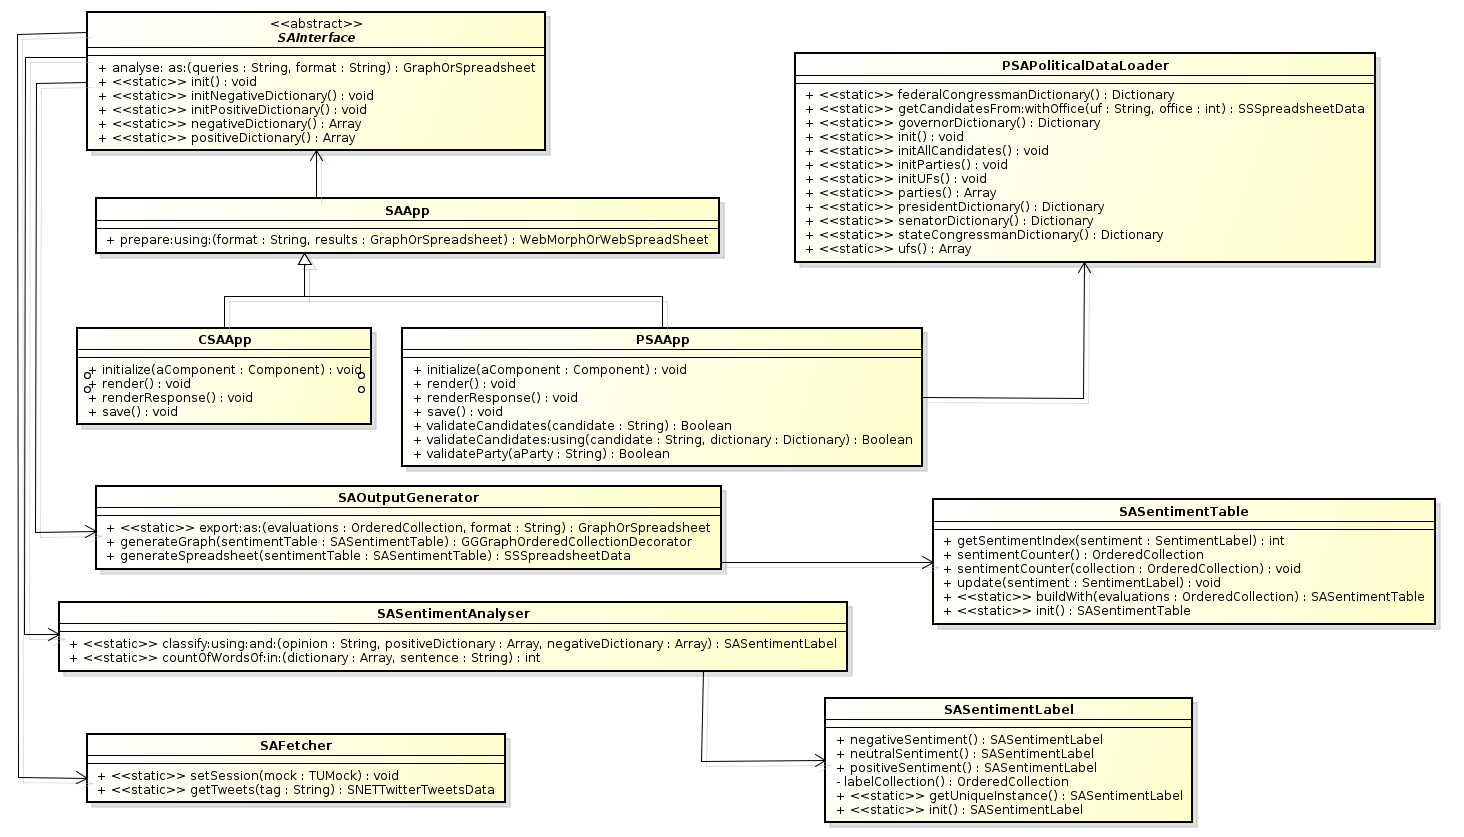
\includegraphics[width=16cm]{figures/UML.png}
\label{fig:uml}
\end{figure}

\newpage
\subsection{Rodando as Aplicações}
Para iniciar as aplicações de Análise de Sentimento basta seguir o simples passo-a-passo abaixo:

\begin{enumerate}
	\item No Squeak, abrir o Seaside Control Panel
	
	\item Dentro dele, clicar com o botão direito e então na opção Add adaptor...
	
	\item Escolher o tipo: WAComancheAdaptor
	
	\item Pressionar o botão ``Start''
	
	\item Abrir o navegador no endereço: localhost:8080/god
\end{enumerate}

Feito isso aparecerá a tela inicial, figura \ref{fig:ini}.

\begin{figure}[h]
\caption{Tela Inicial}
\centering
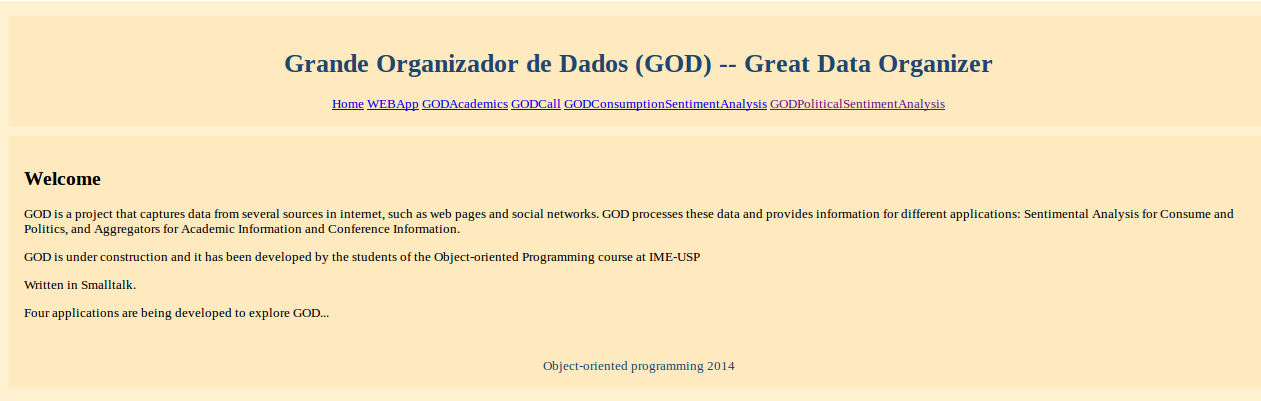
\includegraphics[width=14cm]{figures/inicio.png}
\label{fig:ini}
\end{figure}

\subsubsection{Análise de Sentimento de Consumo}
Para iniciar essa aplicação, basta clicar na opção do cabeçalho GODConsumptionSentimentAnalysis, que então surgirá a tela para pesquisar algum produto, figura \ref{fig:cons-pesq}.

\begin{figure}[h]
\caption{Análise de Sentimento de Consumo}
\centering
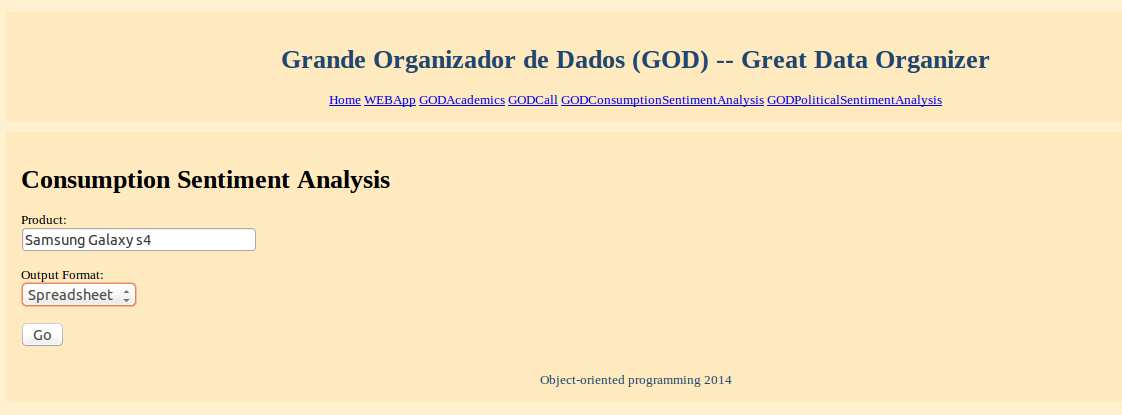
\includegraphics[width=14cm]{figures/consumo-pesquisa.png}
\label{fig:cons-pesq}
\end{figure}

Um possível resultado dessa pesquisa seria, por exemplo, o da figura \ref{fig:cons-result}, mostrado a seguir:

\begin{figure}[h]
\caption{Pesquisa - Galaxy s4}
\centering
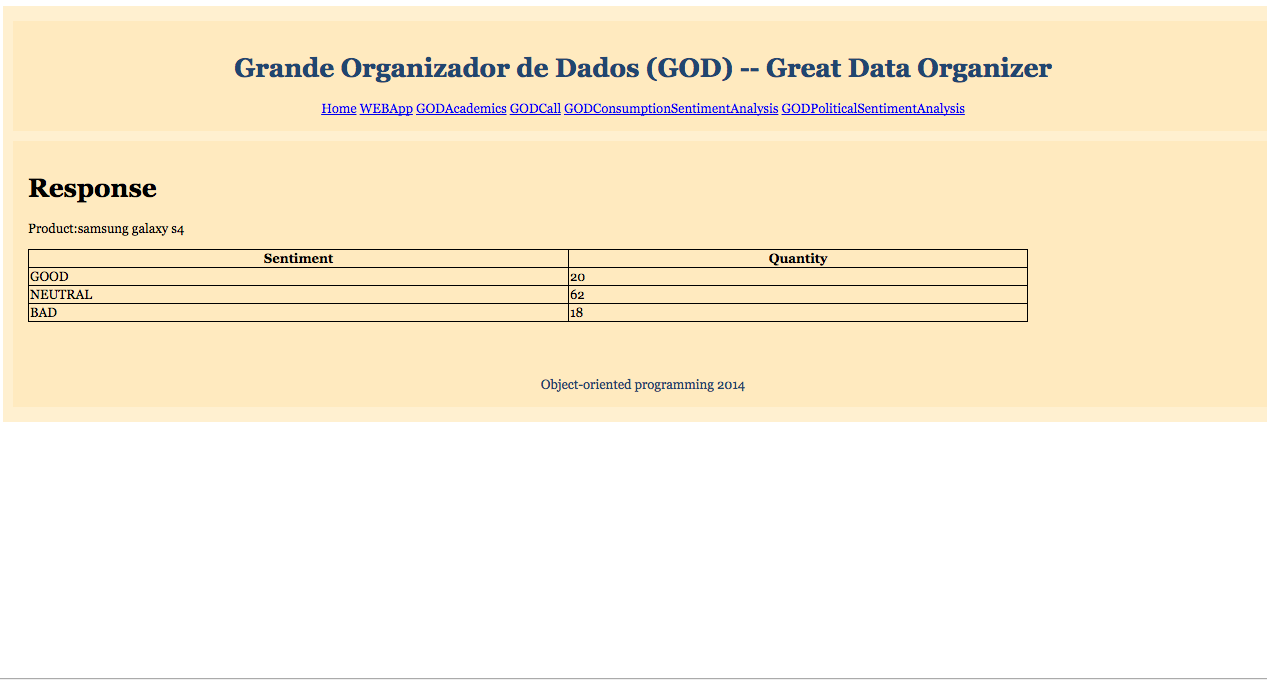
\includegraphics[width=14cm]{figures/consumo-resultado.png}
\label{fig:cons-result}
\end{figure}

\subsubsection{Análise de Sentimento de Político}
Para rodar essa aplicação é preciso selecionar a opção: GODPoliticalSentimentAnalysis, no cabeçalho. Assim, aparecerá a seguinte tela:

\begin{figure}[h]
\caption{Análise de Sentimento Político}
\centering
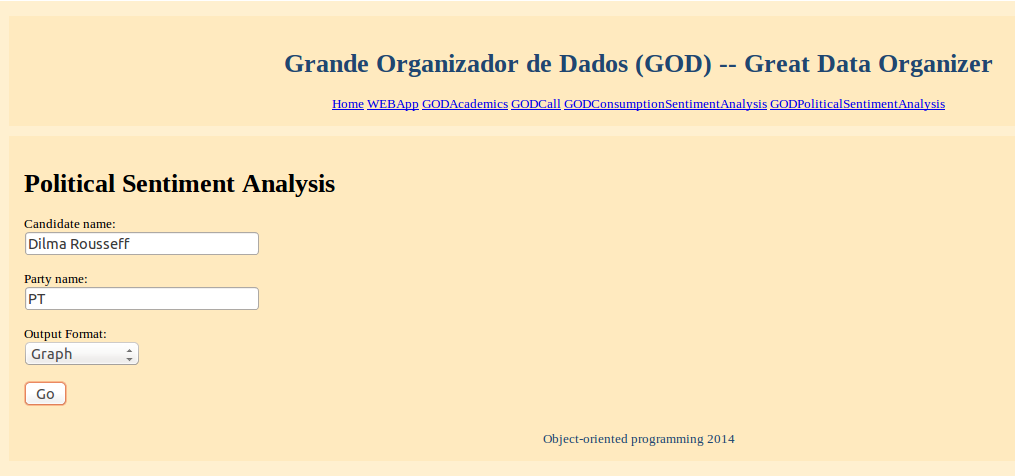
\includegraphics[width=14cm]{figures/politico-pesquisa.png}
\label{fig:pol-pesq}
\end{figure}

Um possível resultado dessa pesquisa seria, por exemplo, o da figura \ref{fig:pol-result}, mostrado a seguir:

\begin{figure}[h]
\caption{Pesquisa - Dilma PT}
\centering
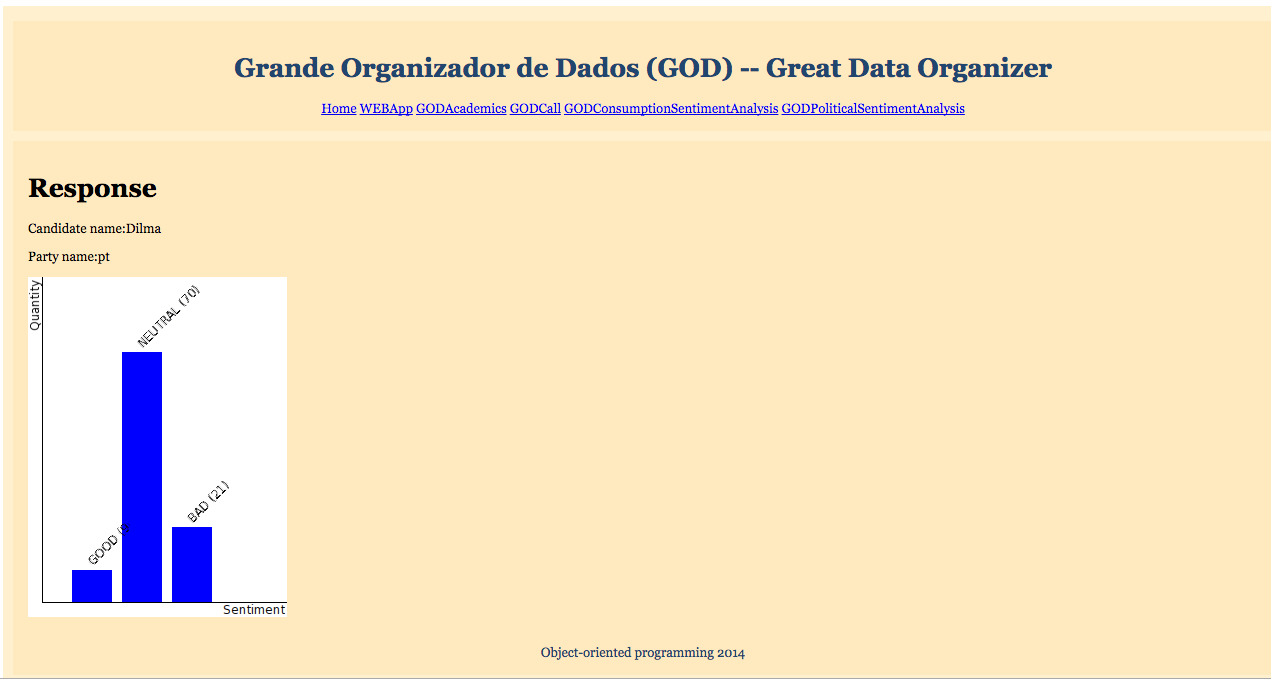
\includegraphics[width=14cm]{figures/politico-resultado.png}
\label{fig:pol-result}
\end{figure}

\newpage

\section{O que falta implementar}
\subsection{Arquivos de texto}
\begin{enumerate}
\item Entrada e saída em DOC
\end{enumerate}

\subsection{Planilhas}
\begin{enumerate}
\item Entrada e saída em XLSX
\end{enumerate}

\subsection{Gráficos}
\begin{enumerate}
\item Saída em gráfico de pizza
\end{enumerate}

\subsection{Agregação de conferências}
\begin{enumerate}
\item Utilização de tags sobre as publicações que devem ser apresentadas em uma conferência
\end{enumerate}
\newpage
\section{Sugestões para requisitos futuros}
\subsection{E-mails}
\begin{enumerate}
\item Enviar arquivos em anexo
\item Enviar emails em html
\end{enumerate}

\subsection{Redes sociais}
\begin{enumerate}
\item Utilizar dados de um usuário de verdade para retornar mais informações do Facebook. No momento, utiliza-se um usuário de teste, o que limita os dados que o Facebook oferece.
\item Salvar no banco de dados, a cada semana, os resultados das buscas mais utilizadas no Twitter, pois ele só retorna tweets de até uma semana atrás nas buscas.
\item Utilizar paginação de resultados para contornar o limite de 100 tweets retornados em buscas do Twitter.
\end{enumerate}

\subsection{Filtros}
\begin{enumerate}
\item Implementar filtros por expressões regulares
\item Filtrar HTML por XPath
\item Filtrar por conteúdo, título, tags e origem ao mesmo tempo
\item Implementar a opção de filtrar os dados que já estão no banco de dados
\item Criar testes com mocks
\end{enumerate}

\subsection{Processadores}
\begin{enumerate}
\item Busca de documentos utilizando tf-idf
\item Utilizar tf-idf para analisar textos
\item Implementar stemming ou lematização para melhorar a geração de tags
\end{enumerate}

\subsection{Banco de dados}
\begin{enumerate}
\item Criação de backups
\item Controle de acesso dos usuários
\end{enumerate}

\subsection{Análise de sentimento de consumo}
\begin{enumerate}
\item Melhorar a análise utilizando relações de uma palavra com outra
\item Adicionar cores ao gráfico (verde para GOOD, amarelo para NEUTRAL e vermelho para BAD)
\item Adicionar cores à planilha
\item Mostrar o gráfico e a planilha na mesma busca
\item Melhorar o layout
\end{enumerate}

\subsection{Análise de sentimento político}
\begin{enumerate}
\item Mostrar planilha e gráfico na mesma busca
\item Utilizar cores para o sentimento da pesquisa (verde, amarelo e vermelho)
\item Adicionar técnicas alternativas de análise, que não utilizem dicionários
\item Criar opção de restringir a análise a um período de tempo (intervalo de tempo, ou primeiro turno das eleições de algum ano)
\item Adicionar autocomplete para candidatos e partidos
\end{enumerate}

\subsection{Agregação de informações acadêmicas}
\begin{enumerate}
\item Realização de busca fuzzy por journals (por exemplo, 'plos comp biology' dá 'plos computation biology')
\item Busca em mais fontes
\end{enumerate}

\subsection{Agregação de conferências}
\begin{enumerate}
\item Implementação de crawling incremental
\item Busca em outras fontes (como o Academic Search da Microsoft)
\item Adição de novas informações (local da conferência, transporte, histórico de clima, pontos turísticos e hotéis na região)
\item Adição de informações acadêmicas (estatísticas sobre os trabalhos apresentados em uma conferência)
\end{enumerate}
\newpage
\section{Instalação}

\subsection{Pré-requisitos}

\subsubsection{Instalação do Magma}
Nesta seção são descritos os requisitos para instalação e instruções principais para trabalhar com a biblioteca.

Para o uso do magma, é recomendável a instalação de uma máquina virtual (Virtual Machine - VM) para lidar com problemas de sistema operacional na parte de persistência de informações (uso de imagens). De uma forma geral, a VM proporciona um ganho significativo de performance.

\subsubsection{Passos de Instalação}

Um modo de instalar é usando o "SqueakMap Catalog" que está em "Apps" na barra de menu do Squeak (ver Fig.~\ref{fig:passo1_InstallMagma1}).

\begin{figure}[!htb]
\centering
\includegraphics[width=0.7\textwidth]{passo1_InstallMagma1.png}
\caption{Instruções para instalação do magma.}
\label{fig:passo1_InstallMagma1}
\end{figure}

Logo, seguir os seguintes passos:
\begin{itemize}
\item{No SqueakMap clique com o botão direito do mouse no quadro esquerdo superior e garantir que todas as opções estejam desmarcadas. Isso permitirá visualizar os pacotes do Magma (Ver Fig.~\ref{fig:passo2_InstallMagma2}).}

\begin{figure}[!htb]
\centering
\includegraphics[width=0.7\textwidth]{passo2_InstallMagma2.png}
\caption{Instruções passo 2.}
\label{fig:passo2_InstallMagma2}
\end{figure}


\item{Clique com o botão direito do mouse no pacote "client" (versão 1.4) do Magma e escolher a opção "install".(Ver Fig.~\ref{fig:passo3_InstallMagmaClient})}

\begin{figure}[!htb]
\centering
\includegraphics[width=0.8\textwidth]{passo3_InstallMagmaClient.png}
\caption{Instruções passo 3.}
\label{fig:passo3_InstallMagmaClient}
\end{figure}


\item{Repetir o ponto 2 para instalar os pacotes  "server" e o "test" do Magma. (Ver Fig.~\ref{fig:passo4_InstallMagmaServer})}

\begin{figure}[!htb]
\centering
\includegraphics[width=0.8\textwidth]{passo4_InstallMagmaServer.png}
\caption{Instruções passo 4.}
\label{fig:passo4_InstallMagmaServer}
\end{figure}

\end{itemize}





\end{document}
